% Authoritative closure source; historical paper generators must not overwrite it.
% Scientific revision dated 30 October 2026; use build-revised-paper.py.
% Historical assets remain fixed. Revised assets/PDF: scripts/build-revised-paper.py.
\documentclass[10pt]{article}
\usepackage[T1]{fontenc}
\usepackage[utf8]{inputenc}
\usepackage{lmodern,microtype}
\usepackage[margin=1in]{geometry}
\usepackage{amsmath,amssymb,amsthm,booktabs,longtable,array,graphicx}
\usepackage[round,authoryear]{natbib}
\usepackage{xcolor}
\usepackage[colorlinks=true,linkcolor=blue,citecolor=blue,urlcolor=blue]{hyperref}
\usepackage{xurl}
\newtheorem{proposition}{Proposition}
\newtheorem{lemma}[proposition]{Lemma}
\newtheorem{corollary}[proposition]{Corollary}
\newtheorem{example}[proposition]{Counterexample}
\newcommand{\A}{\mathcal A}
\newcommand{\TV}{d_{\mathrm{TV}}}
\newcommand{\code}[1]{\texttt{\detokenize{#1}}}
\makeatletter
\let\closureinput\@@input
\makeatother
\setlength{\emergencystretch}{3em}
\setlength{\tabcolsep}{4pt}
\title{Learning Local Coloring Rules:\\Continuation Fidelity, Progress, and Failed Repair}
\author{Research collaboration\\Author list and order pending coauthor agreement}
\date{30 October 2026 --- revised research draft}
\hypersetup{pdftitle={Learning Local Coloring Rules: Continuation Fidelity, Progress, and Failed Repair}}
\begin{document}
\maketitle
\begin{abstract}
Can perfect agreement on a teacher's observed actions conceal an incorrect
local rule? In a distributed coloring framework, three BE/E1 training
procedures agree on every measured native teacher action, yet disagree
sharply when the proposed color or participation message changes. We define
these typed continuations explicitly and audit both occurrence-weighted
accuracy and sufficient local input types. The historical counterfactual
procedure is more accurate, but uses more labels and mostly familiar types;
a separate forty-model, budget-matched experiment tests held-out input types.
GM improves from 50\% to 100\% balanced accuracy when interventions supply
negative color confirmations absent from the native control; autonomous
success is unchanged. BE has an uncertain mean gain and fewer autonomous
successes (7,405 versus 9,204 of 10,000). A post-test eligibility-only
diagnostic scores 99.71\% BA versus CF's 90.41\%, whereas CF has higher
equal-type accuracy (86.94\% versus 81.27\%). The held-out input contexts
mostly reuse logical oracle configurations seen in training.
Frozen transfer exposes a complementary limitation: correct rejection can
coexist with stalled proposals or an omitted scheduled repair. On copied
failure witnesses, one-component interventions distinguish these mechanisms
from an incorrect collision veto. Conditional arguments explain why
confirmation fidelity alone guarantees neither progress nor completion.
Native functional coverage of seven teachers and three architectures supplies
context under heterogeneous finite protocols; it does not identify a
universally correct or uniformly superior learned algorithm.
\end{abstract}

\section{Introduction}
Two adjacent pending vertices repeatedly propose the same free color. Their
learned collision veto correctly rejects both, yet the execution reaches its
horizon without finishing. In another learned policy, a scheduled repair
proposes an occupied color; a correct rejection leaves the original conflict
unrepaired because the schedule does not retry. These are observed frozen
transfer failures in our coloring framework. They motivate asking which
local rule a policy learned, beyond whether its usual runs end properly.

A second example makes the identification problem sharper. On the observed
teacher states, passive, matched and counterfactual BE/E1 procedures each
match every measured native action. On the same states with typed proposal
interventions, their responses differ dramatically. A successful native
choice constrains the accepted option but need not determine what happens
to an occupied option or a silent root. Repeated graph testing alone cannot
resolve that ambiguity.

We make three concrete contributions. First, we specify continuation targets
for seven implemented teachers, locating interventions between two learned
communications and accounting for the supplied interpreter. Second, we
reconstruct a paired continuation diagnostic, expose its class imbalance and
local-type overlap, and add a separate prospective comparison with equal
supervised-target budgets and held-out sufficient COMMIT input types. We
quantify what that split withholds, class coverage and programmed diagnostic
controls; it is not a test of new logical conditions. Third, we
connect frozen proposal/repair failures to their missing progress hypotheses
using one-component interventions on preserved witness executions. These
are claims about specified finite experiments and interfaces, not a new
fastest coloring algorithm, general learning theorem, or architecture ranking.

\paragraph{Relation to previous work.}
Neural graph coloring predates this study \citep{lemos2019coloring}, as do
graph-algorithm execution with MAX aggregation \citep{velickovic2020execution}
and trace-based reasoning benchmarks \citep{velickovic2022clrs,velickovic2021nar}.
DAgger addresses learner-induced state distributions \citep{ross2011dagger};
causal confusion in imitation already motivates interventions
\citep{dehaan2019causal}. Our fixed-bank teacher continuations are not a new
formulation of these general ideas. GNN/local-computation connections and
information restrictions are established
\citep{loukas2020depth,sato2019approximation}. Alignment and schedules affect
extrapolation \citep{xu2021extrapolate,mathys2023flood}; asynchronous robustness
requires its own assumptions \citep{solodova2025hogwild}, which we do not test.
Recent coloring methods learn parallel orderings \citep{langedal2025ordering},
use recursive warm starts \citep{vanderbush2026warm}, or learn contrastive
coloring geometry with transfer \citep{le2026contrastive}. Recent sufficient
conditions for provable algorithm learning \citep{wittig2026which} go beyond
our finite extrapolation evidence. Our specific increment is the combination
of scoped teacher interfaces, paired continuation diagnostics and replayable
failure mechanisms, rather than neural coloring or size transfer themselves.
Hint-ReLIC already regularizes algorithmic predictions across input
augmentations preserving the next trace step \citep{bevilacqua2023causal};
we instead acquire explicit teacher-continuation labels under alternative
messages, whose targets can change. No-hint reasoning already separates
terminal learning from trajectory imitation \citep{rodionov2023without}.
We claim neither algorithmic intervention nor that distinction as new.
Appendix~\ref{app:related} compares candidate contributions with precedents.

\section{Interfaces and Continuation Targets}
We use finite simple undirected labeled graphs $G=(V,E)$, $n=|V|$,
$d(v)=|N(v)|$ and maximum degree $\Delta$. Native training uses $\Delta\le3$
and $C_v=\{0,1,2,3\}$. Transfer uses either the global list
$C_v=\{0,\ldots,\Delta\}$ or local initial segments
$C_v=\{0,\ldots,d(v)\}$. These are not arbitrary list-coloring instances.
Partial colors satisfy $x_v\in\{-1\}\cup C_v$, where $-1$ is pending.
Availability is $\A_v=C_v\setminus\{x_u:u\in N(v),x_u\ne-1\}$.

A teacher is a specified state machine with observations, private inputs,
phases and an interpreter. The learned policy receives declared observations
and emits decisions; the interpreter applies them. Anonymous trials use two
neighbor exchanges; ColorTrials communicates availability-dependent
preferences in the second. JP and Greedy need one exchange mathematically,
but their neural decomposition retains two. GM has supplied blocks, barriers
and a serial repair queue; BE supplies algebraic predicates and a reduction
clock. These are distinct computational regimes, not equal-cost anonymous
LOCAL algorithms. Message length and palette computation grow with palette
size; we make no CONGEST complexity claim.
Recorded native steps count state-machine applications. BE has two
point-reduction steps and thirteen KW steps; neural point decisions use the
first exchange, whereas KW evaluates the second stage as well. Fifteen
native steps are not a fifteen-round learned communication complexity bound.

Mathematical random statements use fresh independent ideal draws.
Implementation uses namespaced PCG64 streams and float32 observations.
Required IDs are fixed distinct integers in $\{0,\ldots,65535\}$. The
implementation restricts $1\le n\le65536$, including anonymous experiments
for convenience; this is not an anonymous-algorithm size lower bound.

\paragraph{Evaluation objects.}
Functional success means a complete proper in-list coloring within the
protocol horizon and satisfaction of checked native invariants. A cutoff
is a benchmark failure, not proof of nontermination. Action fidelity compares
common states/private inputs. Transition fidelity compares updated states;
different action codes need not yield different transitions. Continuation
fidelity evaluates a declared oracle $O_T(S,a)$ after a typed message or
color-query intervention. Such messages need not be sampled by the native
teacher. Execution costs use teacher-specific units. Distributional fidelity
concerns the full terminal vector and status on a fixed labeled graph.
Terminal validity alone does not imply any of the other properties.

\paragraph{A continuation is a specified target, not an inferred intention.}
Fix a legal teacher-prefix state $S$, including its phase, permissions $w$,
IDs, slots, private inputs and derived algebraic data. After the first
exchange, a rooted query supplies typed messages $(p_u,c_u)$ at the root and
its neighbors: $p_u\in\{0,1\}$, $p_u\le w_u$, $c_u\in C_u$ (four option
indices for KW). Let $F_v(c)$ mean that the queried color, or the decoded
receiver-relative KW option, is unoccupied. Define
\[
 E_v=\begin{cases}
 w_v\,\mathbf1[\text{no pending neighbor has a larger ID}],&T=\mathrm{JP},\\
 w_v\,\mathbf1[a_v\ge q],&T=\mathrm{BE}\text{ in KW},\\
 w_v,&\text{otherwise}.
 \end{cases}
\]
The binary confirmation oracle is
\begin{equation}\label{eq:oracle}
 O_T(S,p,c)=E_v p_v F_v(c_v)\,R_T(S,p,c),
\end{equation}
where $R_T$ is the rule-specific condition below. It returns a confirmation
bit; it does not select a new color, repair an invalid proposal, or promise
progress. Its agreement with the native decision is checked when $p,c$ are
the native messages. Off-policy targets are defined by this extension of the
rule, rather than uniquely identified by the original native trace.

\begin{table}[htbp]\centering\small
\begin{tabular}{p{.18\linewidth}p{.38\linewidth}p{.35\linewidth}}
\toprule Rule & $R_T$ and separate targets & Legal state and permitted intervention \\
\midrule
Luby, Johansson & No active neighbor offers $c_v$ & Proper partial state;
replace typed participation/candidate messages after first exchange \\
JP & No active neighbor offers $c_v$ & Proper partial state; fixed coherent
distinct IDs. New ID assignments precede replay, not independent edge edits \\
ColorTrials & Root preference for $c_v$ strictly exceeds every writable
neighbor's preference when that color is free there & Proper partial state;
preferences and their availability-dependent messages stay coherent.
Silencing $p_u$ does not remove that neighbor's preference message \\
BE & $R_T=1$ in KW. LINIAL has a separate legal-point target & Proper
auxiliary coloring from validated reduction prefix; change option query,
not polynomial evaluations, equalities, clock or bounds \\
GM, Greedy & $R_T=1$ in color phases. GM DETECT separately marks the
smaller-ID endpoint of each equal-color/equal-slot edge & Scheduled
prefix; GM allows legal temporary same-slot conflicts. Repair queue follows
marks. Replace P/C without independently editing marks or queue \\
\bottomrule
\end{tabular}
\caption{Self-contained continuation contracts. The main experiments use
rooted message queries, not arbitrary edited global states. Alternative
prefixes must satisfy the teacher's native safety/schedule constraints.}
\label{tab:contracts}
\end{table}
For ColorTrials the competing preference is $-1$ when the neighbor is not
writable or its queried color is occupied; strict comparison includes ties
as rejection. For GM, $F_v$ is computed against actual speculative colors,
including during repair. DETECT does not use a P/C continuation label.
For BE, a queried index $c$ decodes to $(B-1-a_v)4+c$ at a high auxiliary
color, with $q=\lceil4B/5\rceil$. Low colors cannot recolor. LINIAL predicts
an unblocked evaluation point; the interpreter computes the corresponding
polynomial value. This supplied arithmetic is not learned.

\paragraph{Worked KW continuation.}
A replayed training witness has $B=7$, $q=6$, root auxiliary color $a_v=6$
and neighbor auxiliary colors $3,0,1$. Its four decoded options are
$0,1,2,3$, so only option index 2 is free. With $w_v=p_v=1$,
$O_{\rm BE}(S,p,c_v=2)=1$ and $O_{\rm BE}(S,p,c_v=1)=0$; setting $p_v=0$
also gives zero. The state, clock and neighbor equalities are identical in
the three queries. Native imitation sees the successful choice 2; it need
not constrain rejection of choice 1 or silence. The source is seed 94101,
root 0, native step 12, tape 14094519662940050106; its full legal prefix is
stored with the original acquisition witnesses.


\section{Teachers and Learned Communication}
\label{sec:teachers}
Names identify the implemented variants. Bibliographic names identify source
families, not guarantees imported without checking the variant.
Appendix~\ref{app:teachers} specifies rules and conditional guarantees.
\begin{table}[htbp]\centering\small
\begin{tabular}{p{.16\linewidth}p{.40\linewidth}p{.35\linewidth}}
\toprule Teacher & Exact rule & Supplied information/computation \\
\midrule
Luby & Participate with probability $1/2$, propose uniformly available,
veto equal active offers & Pending/fixed colors, two private draws; anonymous \\
Johansson variant & Always active, uniform available proposal, equal-offer
veto & Anonymous observations; no imported triangle-free theorem \\
ColorTrials & Minimum strictly winning available color, else wait & Four
private preferences in $\{0,\ldots,3\}$ natively; two exchanges \\
JP & Pending strict ID maximum writes first-fit & Coherent relative ID
comparisons; fixed IDs \\
BE\_BASE\_D3 & Two polynomial reductions, thirteen KW reductions & Bounded
IDs, fields $13,7$, point/option equalities, bound/target and phase interpreter \\
Speculative GM & Four-block first-fit, same-slot marks, serial repair & IDs,
slots, permissions, phases, queue built from predicted marks \\
Greedy & First-fit in increasing-ID permutation & One externally scheduled
write permission per step \\
\bottomrule
\end{tabular}
\caption{Native teachers and distinct information regimes. ColorTrials is
the repeated strict-preference subroutine; GM temporary conflicts are legal.}
\label{tab:teachers}
\end{table}

\paragraph{Shared communication.}
E1 NORMALIZED uses node/color MLPs, learned availability, private-input
participation, a normalized ordered palette-prefix scorer and learned COMMIT
after a second MAX exchange. DeepSets replaces mainly the palette scorer by
shared color features and mean palette context. LocalPaletteTransformer uses
two-head attention inside each node's palette. Both retain learned graph
communication. Functional palette positions are supplied; color-renaming
equivariance is not assumed. Hidden/message widths are $64/32$. Canonical
E1/DeepSets/Transformer have 16,035/17,907/16,995 parameters. Native residual
adapters give 19,396/21,268/20,356 where required.

Learned components include participation, proposal scores and confirmation,
BE point/option decisions, and GM marks. Polynomial evaluation, schedule
construction, decoding, list-membership masks and fixed-order argmax are
supplied. There is no exact availability mask, winning flag, eligibility
decision or collision veto in neural inference. GM's queue follows predicted
marks; an exact teacher never repairs the student's rollout.

\begin{figure}[htbp]\centering
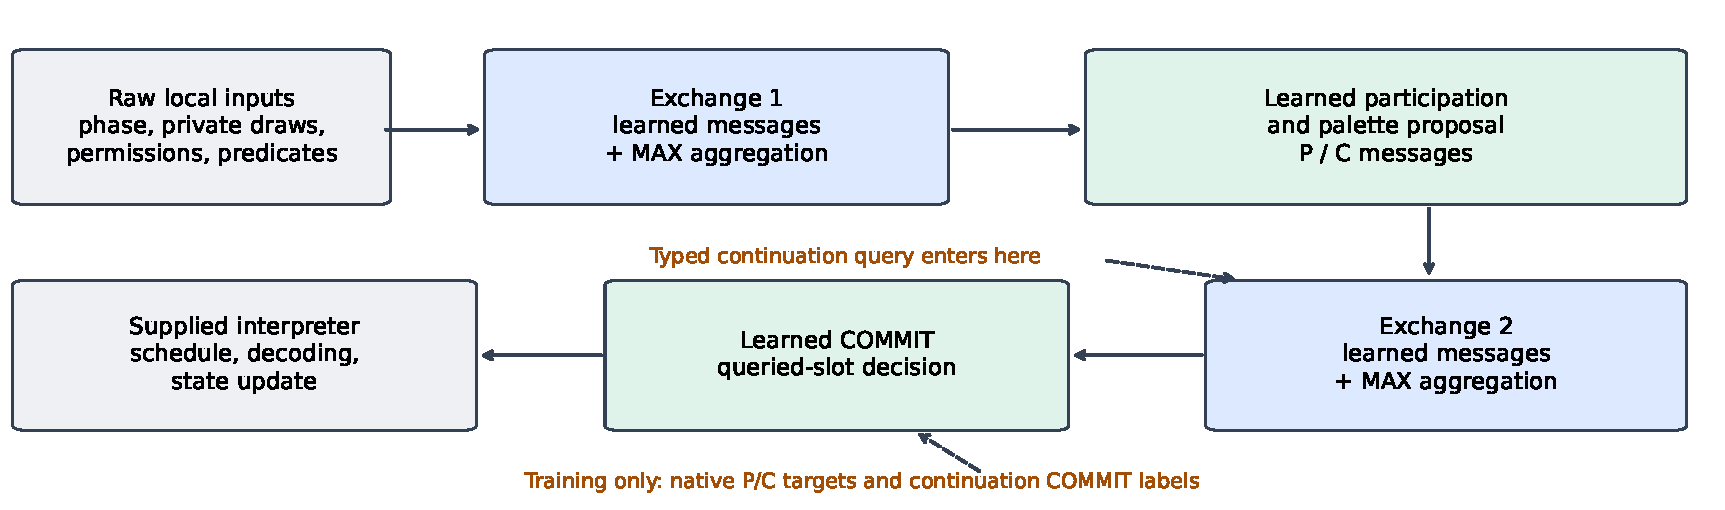
\includegraphics[width=\linewidth]{figures/revision-architecture.pdf}
\caption{Two learned neighbor exchanges inside a supplied state machine.
Each color slot shares parameters; graph messages use MAX. Dashed arrows
locate supplied training targets and diagnostic queries. No continuation oracle or exact
availability filter participates in an autonomous learned rollout.}
\label{fig:architecture}
\end{figure}
The first exchange consumes raw pending/own-color predicates and declared
phase, permission, relative-order or algebraic-equality context. Learned
features feed participation and palette scores. The second exchange consumes
typed P/C messages and raw color predicates, then reads the queried slot's
COMMIT logit. ColorTrials instead exchanges per-color preference/features
and selects its candidate after that exchange. GM DETECT queries the current
color to predict a mark. Hidden-state transformations and message functions
are learned; the interpreter supplies scheduling, list positions, action
decoding, program color/auxiliary updates and phase/queue advancement.
This decomposition locates the continuation query precisely and separates
learned decisions from the externally provided computation.


\paragraph{Variable-degree representation.}
The historical serializer fixes four colors and three neighbor positions.
Frozen transfer evaluates the same shared tensors with a sparse structural
adapter. Native parity controls cover 21,630 decisions for 150 extensible
selected/control checkpoints: no hard-action differences were observed,
maximum absolute logit discrepancy $1.526\times10^{-5}$. Separately, 1,170
native executions cover all 195 original selected/control checkpoints.
These are finite checks, not bitwise-equivalence proofs for every kernel.
ColorTrials uses preference/$\Delta$ in transfer, agreeing with preference/3
natively; the out-of-domain scaling choice matters.
For native-context teachers, participation averages first-stage features
over each receiver's valid palette slots in the structural adapter. Fixed
tensors therefore still use an explicitly adapted computation outside the
historical serializer; palette membership is not the only adaptation.

\section{Supervision and Experimental Comparisons}
\label{sec:learning}
Native training samples sizes 8, 12, 16, 24 at degree at most three and
global $K=4$. Historical banks use six graph families; new banks add
edgeless, mixed-component and clique/isolate examples. States, observations
and optimization are part of each cohort's identity.

Let $P,C$ denote participation/candidate messages. Passive training
supervises native components on teacher prefixes. Its COMMIT loss evaluates
the model's current messages against a stored native label, which may be
inconsistent with the correct continuation for those messages. Matched
training evaluates stored teacher $P,C$ with their concordant native label,
without acquiring new labels. Counterfactual training uses the same native
bank plus four stored COMMIT labels per color root: it cycles the queried
root through four colors with teacher-specific message interventions and a
silence case. After matched warmup, its loss is
\[
L=L_P+L_C+\tfrac12L_{\mathrm{native,matched}}+
\tfrac12L_{\mathrm{continuation}}.
\]
LINIAL point and GM DETECT phases retain their native losses. These fixed
teacher-state banks differ from collecting states visited by the learner.

Paired arms share architecture, seed, initialization, native data, minibatch
order, Adam learning rate $10^{-3}$ and batch size 64; at a fixed milestone
they share updates. CF adds labels and changes the confirmation loss
distribution. Thus matched versus CF does not identify an intervention-only
effect or efficiency at equal total label budget. Acquired component labels,
model access, presentations, updates, bytes and CPU time are separate costs.
Replaying a stored label is optimization, not new supervision. Shared banks
are charged once for physical acquisition, separately for each model's access.

\paragraph{Admissibility.}
Anonymous queries require proper partial prefixes. JP signs derive from a
coherent fixed ID order. BE states come from legal polynomial/KW replay;
derived predicates cannot be edited independently. GM requires legal
speculative history and schedule. A typed rooted continuation need not form
a jointly consistent graph-wide intervention. We claim neither arbitrary
state robustness nor joint intervention fidelity from root queries.

\paragraph{Selection and replication.}
The historical sample-budget study has seven budgets $10^3$--$10^6$,
500 updates and five seeds: 735 policies. New procedures record 500, 1,500
and 4,000-update milestones. A prospective amendment expands development
from 60 to 300 runs before new confirmation. Five candidate hashes and a
final namespace are frozen before a once-only 1,000-run battery per policy.
Failed candidates remain; subsequent follow-ups use new namespaces. Local
registration is supported by Git/artifact provenance, not independently
timestamped external preregistration. Appendix~\ref{app:training} supplies
the budget/provenance table and costs.

\section{Native Agreement and Continuation Fidelity}
\label{sec:cf}
We reconstruct the existing paired 4,000-update diagnostics on 60 exact
teacher trajectories at sizes 28 and 36 per seed. Their graph/tape namespaces
are disjoint from training. They belong to the repeatedly used development
split, not an untouched final fidelity battery.
BE/E1 gives 28,800/28,800 native permitted-root action agreements in every
arm and seed, but very different continuation responses:
\begin{table}[htbp]\centering\small
\begin{tabular}{lrrrr}
\toprule Procedure & Labels & Mean acc. (\%) & Seed range (\%) & Mean BA (\%) \\
\midrule
\closureinput tables/closure-be-summary.tex
\bottomrule
\end{tabular}
\caption{BE/E1, 4,000 updates. Each seed has 99,840 continuation queries.
Means describe five paired training seeds; 499,200 queries per arm are
correlated within states/trajectories, not independent training replicas.
BA averages sensitivity and specificity within seed, then over seeds.
Eligibility-only accepts iff the root is KW-eligible and participating;
these semantic baselines are diagnostics, not trained competitors.}
\label{tab:be}
\end{table}
The paired initial hashes, native arrays, visit counts and final minibatch
RNG states agree. CF adds 3,776 labels, changes COMMIT contexts and splits
its confirmation loss. This supports a difference between the full
procedures, not an intervention-only effect, sample efficiency, or universal
functional improvement.
Only 2.7774--3.1200\% of queries are positive. Every arm has zero false
negatives; CF has 34 false positives, all on eligible but silent roots.
Most of the raw gap concerns rejection of ineligible KW continuations.
Among eligible active queries (4,150--4,598 occurrences per seed), CF is
100\% correct in all seeds, whereas passive and matched accept every option,
including occupied ones: mean accuracy 67.8117\%, BA 50\%. Thus the effect
also includes learning to reject occupied options, not only a redundant
eligibility gate. Always rejecting is accurate overall but destroys progress.

\paragraph{Novelty of the evaluation queries.}
Reconstructing the original query RNG reproduces every numerator. Only 91
of 499,200 occurrences exactly match a complete serialized training query.
However, BE COMMIT discards many serialized fields. Its queried-slot logit
depends on phase, permission, signed KW offset, root participation, and the
MAX-set of occupied/participating/offering neighbor types. Between 99.277\%
and 99.540\% of diagnostic occurrences have one of these sufficient input
types already in training. The four queried colors and intervention families
are not held out.
Among the 549, 459, 717, 522, 722 occurrences with unseen sufficient types,
CF correctness is 549, 437, 717, 510, 722, versus matched
158, 342, 229, 182, 246. This posthoc restricted result preserves a seed-wise
advantage. Its correlated small subsets and development reuse do not support
broad new-intervention-distribution generalization. Appendix~\ref{app:cf}
defines the sufficient-input key and gives per-seed numerators.
These unseen-type subsets include 52,108,90,56,60 positives and both classes
in every seed. All three arms accept all positives; CF's advantage is again
specificity on negative continuations. The mean unseen-subset BA is
99.1157\% CF versus 66.5299\% matched and 50\% always-reject.

\begin{figure}[htbp]\centering
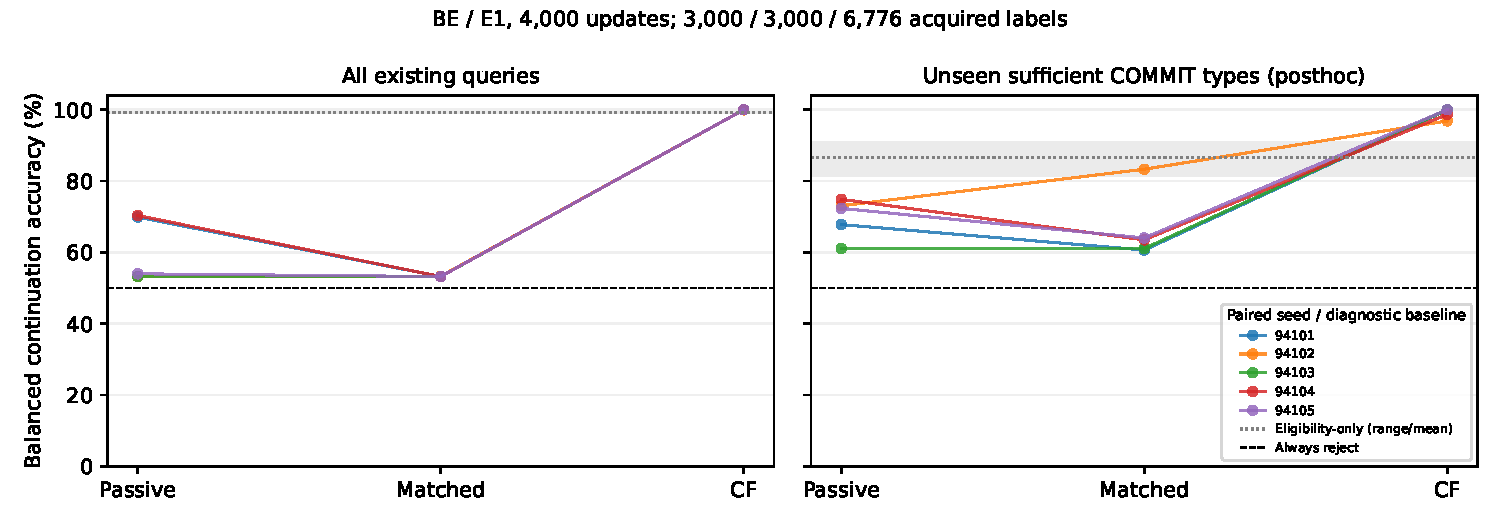
\includegraphics[width=.96\linewidth]{figures/closure-counterfactual.pdf}
\caption{BE/E1 balanced accuracy across paired seeds, with constant-reject
and eligibility-only diagnostic baselines. Right: posthoc unseen sufficient
COMMIT types. Curves connect treatments within each paired seed;
label budgets differ by arm.}
\label{fig:cf}
\end{figure}

\paragraph{Equal weight per sufficient local type.}
Occurrence-weighted accuracy gives frequent local configurations more weight.
We additionally average accuracy within each sufficient COMMIT input type and
then over distinct types, separately within each training seed. This measures
the tested type set, not a natural input distribution or a new training replica.
Reconstruction with the original RNG and 256-root chunks reproduces every
historical numerator before this reweighting.

\begin{table}[htbp]\centering\small
\begin{tabular}{lrrr}
\toprule Procedure & Occurrence acc. (\%) & BA (\%) & Equal-type acc. (\%) \\
\midrule
passive & 22.640 & 60.141 & 50.784 \\
matched & 9.269 & 53.254 & 46.350 \\
counterfactual & 99.993 & 99.996 & 99.488 \\
always reject & 97.046 & 50.000 & 82.317 \\
eligibility only & 98.599 & 99.278 & 78.973 \\
\bottomrule
\end{tabular}
\caption{Same historical BE queries, three different estimands. Entries
average five paired seeds. Equal-type accuracy weights the 115--132 distinct
tested types equally within seed, rather than their 99,840 occurrences.}
\label{tab:type-weighting}
\end{table}

These estimates retain both the strong rejection difference and the limits
of the familiar-type diagnostic. Per-seed seen/unseen, eligibility, silence
and occupied/free strata, including all confusion counts, accompany the
type-level occurrence counts in the revision evidence. The split uses the
union of native and stored CF training types in all historical arms, making
its novelty criterion common rather than treatment-dependent.


\paragraph{Other teachers and dependent architecture comparisons.}
At the same milestone GM/E1 has mean continuation accuracy 75.3632\% for
passive/matched versus 100\% CF; CT has 96.6570\%, 97.2439\%, 99.7452\%.
Their denominators vary by seed. These are supporting diagnostics.
Paired BE/GM CF COMMIT tensors are identical across the three palette cores
at audited milestones: fixed-proposal second-stage losses do not involve
their palette scorer. These are five paired confirmation replicas per
milestone, not fifteen independent architecture replicas. CT couples
second-stage gradients to proposal scoring and lacks that tensor identity.

The scoped answer is positive: this CF procedure better reproduces these
typed teacher continuations, including some unseen local types, even when
passive native agreement is already perfect. It is not always necessary,
universally functionally superior, or shown more label efficient. The historical comparison remains separate from the new budget-matched
experiment below.

\section{Prospective Equal-Budget Continuation Experiment}\label{sec:prospective}
We test a separate acquisition-strategy contrast with BE/E1 and GM/E1
(19,396 parameters). Ten fresh paired seeds per teacher give forty models.
Before training, a fixed SHA256 partition holds out 20\% of sufficient
queried-slot COMMIT type buckets, common across seeds. Phase, root/context
features and distinct neighbor message types determine this key; MAX removes
multiplicity. Neither training arm supervises a held-out continuation type.
LINIAL and DETECT remain separate native targets. This is a split of input
contexts within the same intervention templates. It does not withhold all
coarser oracle-relevant configurations (quantified below).

Each pair shares 3,000 native component targets and 3,600 fresh auxiliary
rooted states. On each auxiliary state the native arm acquires one native
COMMIT target and CF one prespecified intervened COMMIT target. Both queries
must pass the training-type filter to retain that state. GM auxiliary quotas
are 1,800 ASSIGN and 1,800 REPAIR; BE uses KW only. Each model therefore
accesses 6,600 optimization targets. Native P/C conditioning is supplied to
both arms equally and charged separately: 7,200 root values plus retained
neighbor values. Simulator computation, rejected states and duplicate queries
are also recorded; this does not equate all teacher-computation costs.
The root option cycles through native-option offsets 0,1,2,3 modulo four.
Participation is the root permission, except that offset three independently
silences it with probability 1/4; neighbor messages remain native. The cursor
advances before filtering, including discarded roots. Test queries use the
same intervention and retain held-out CF types; their phase quotas are
4,000 KW or 2,000 each ASSIGN/REPAIR. This single-query design differs from
the historical four-query diagnostic. Appendix~\ref{app:prospective-method}
specifies the key, serialization, hash and acquisition order.

Adam, batch 64 and 1,500 updates are fixed before test, with 100 matched warmup
updates and the same subsequent native/auxiliary loss weighting. Paired data,
initialization, index sequences and first-stage final tensors agree. All forty
weights are frozen before generating 4,000 held-out queries per seed/teacher
on sizes 28/36 and evaluating 1,000 autonomous runs per model on sizes 32/48/64.
All exact references pass. Every final continuation has zero intersection
with its training sufficient-type set; both truth classes occur in every seed.


\begin{table}[htbp]\centering\small
\begin{tabular}{lrrlc}
\toprule Teacher & Native BA & CF BA & Paired difference [95\% interval] & Successes N / CF \\
\midrule
BE & 84.64 & 90.41 & +5.77 [-13.73,+25.26] & 9,204 / 7,405 \\
GM & 50.00 & 100.00 & +50.00 [+50.00,+50.00] & 10,000 / 10,000 \\
\bottomrule
\end{tabular}
\caption{New final experiment. BA is a percentage; differences and intervals are percentage points,
averaged over ten paired training seeds. Intervals bootstrap paired seeds
(10,000 resamples), conditional on this fixed split/protocol; individual
queries are not independent replications. Success totals are out of 10,000
autonomous runs per teacher/arm. No checkpoint selection uses these tests.}
\label{tab:prospective}
\end{table}

GM equal-type accuracy is 35.44\% native and 100.00\% CF; both arms average 26.01 native steps.

GM gains 50 percentage points in every paired seed without changing any
autonomous outcome or mean step count. Its degenerate bootstrap interval
reflects those identical observed seed differences, not certainty over all
future types or training replicas. BE's mean difference is +5.77 points, but
the interval spans zero (\(-13.73,+25.26\)). BE equal-type accuracy increases
from 51.70\% to 86.94\%, while the two endpoints weight errors differently.
CF adds false negatives in two BE seeds and reduces autonomous successes from
9,204 to 7,405; one further seed has identical failures in both arms.
Mean step counts over \emph{all} final runs (14.53 native versus 13.43 CF)
include early exits on failure. Every successful BE run takes 15 native
steps in both arms; the lower overall mean is not a successful-run speedup.
These are substantive negative results for a uniform-benefit claim.

\paragraph{Post-test diagnostic controls.}
The primary endpoint and all original outcomes above are retained.
The following controls and support audit were added after inspecting the test;
they are descriptive checks, not a revised primary analysis. The programmed
rule $G_v=E_vp_v$ uses supplied eligibility and root participation and ignores
query occupancy. It requires no training and is a diagnostic, not a learned
label-efficiency competitor.

\begin{table}[htbp]\centering\small
\begin{tabular}{llrr}
\toprule Teacher & Procedure & BA (\%) & Equal-type acc. (\%) \\
\midrule
BE & Native & 84.64 & 51.70 \\
BE & CF & 90.41 & 86.94 \\
BE & Eligibility/participation & 99.71 & 81.27 \\
GM & Native & 50.00 & 35.44 \\
GM & CF & 100.00 & 100.00 \\
GM & Eligibility/participation & 53.03 & 62.34 \\
\bottomrule
\end{tabular}
\caption{Same final queries and sufficient-type key; means over ten seeds.
The programmed diagnostic ignores occupancy. BA averages sensitivity and
specificity; equal-type accuracy first averages within each distinct
type, then across types within seed. The diagnostic is post-test.}
\label{tab:prospective-controls}
\end{table}

For BE, the programmed rule scores 99.71\% BA, above CF's 90.41\%,
whereas CF scores 86.94\% equal-type accuracy versus 81.27\%.
A single negative type accounts for 95.05--96.30\% of each 4,000-query bank.
Class balancing therefore leaves the negative subtypes highly imbalanced;
high occurrence-level BA alone does not identify the occupancy condition.
Among eligible active BE queries, native and the programmed rule accept
995/995 free options but reject 0/228 occupied options.
CF rejects 228/228 occupied options but accepts only
814/995 free options. These are pooled descriptive counts over
ten banks, not independent training replications. Appendix~\ref{app:prospective-audit}
reports the full confusion strata.

GM's native control receives 4,344--4,354 positive COMMIT labels and zero
negative COMMIT labels in ASSIGN/REPAIR per seed, while CF receives
1,038--1,098 negatives and the test has 2,420--2,491 negatives per seed.
The native model accepts all test queries, giving BA 50\%; the contrast
therefore demonstrates learning rejections absent from native color supervision.
DETECT has separate positive/negative conflict supervision and is excluded
from these color-label counts. This result does not compare CF with another
acquisition strategy supplying informative negative confirmations.

\paragraph{Support of the held-out queries.}
There are 17--23 distinct sufficient test types per BE seed and 82--92
per GM seed, despite 4,000 occurrences. For these color oracles
$O_T=E_vp_v(1-o_v)$, with $o_v$ the queried-option occupancy. A coarser
configuration $(\text{phase},E_v,p_v,o_v)$ is therefore oracle-sufficient.
CF training has already seen configurations covering 99.475--100.000\% of BE
test occurrences and 100\% of GM test occurrences. The original fine-key
holdout remains disjoint: novelty is defined by contextual combinations
rather than by this coarser configuration. There is no separate evaluation
restricted to novel logical conditions. These tests do not establish extrapolation to new logical
conditions. Per-seed support counts and logical overlap are in
Appendix~\ref{app:prospective-audit}; no split, label or model was changed.

\paragraph{Two distinct BE failure diagnoses (post-test).}
In the two deteriorated CF seeds, 105001 and 105008, COMMIT BA on the 3,600
acquired auxiliary queries is 99.510\% and 100.000\%, versus 52.756\%
and 52.094\% on the held-out contexts. Both models visited all auxiliary
queries. Failure to fit acquired labels alone does not explain these cases:
the observed COMMIT gap concerns generalization across contexts, without
identifying its optimization cause or an architectural impossibility.

Seed 105010 has a different defect: both arms complete only 204/1,000 runs,
despite final COMMIT BA 99.451\% native and 99.949\% CF. Their shared
first stage omits participation on 13/118 eligible test roots.
A replay of the original 32-case cohort localizes the first invariant
violation in one selected run: at KW step 7, vertex 31 must
recolor as the bound drops from 21 to 17, but remains at 17
because participation is false. Its proposed value 12 is free;
changing only root participation makes COMMIT accept it. Thus this state
exposes an upstream omission, rather than an incorrect veto of the actual
silent message. These are selected post-test diagnostics, without retuning,
a continued rescue rollout or an estimate of causes across all failed runs
(Appendix~\ref{app:be-failure-diagnostics}).


The primary endpoint concerns held-out continuation types; autonomous success
is secondary. This finite comparison concerns the specified acquisitions at
equal target/context access. It supports neither extrapolation to new logical
conditions nor an advantage over alternative informative-negative acquisition
strategies. BE's occurrence-level endpoint must be read with its diagnostic
baseline and type weighting; GM's control lacks negative color confirmations.
No universal CF superiority, minimum sample complexity or all-source teacher
efficiency follows.
The protocol, forty checkpoints, all seed outcomes, per-component costs and
freeze receipts accompany the new results (Appendix~\ref{app:prospective}).


\section{Frozen Transfer and Failure Mechanisms}\label{sec:generalization}
The domain-wide totals below are retained from the original closure study.
Its complete raw delivery is unavailable here, so these totals are not a new
independent regeneration. All 225 checkpoint identities have been recovered
by SHA256 from earlier public archives. The new interventions below reconstruct
two selected first-failure cohorts directly with those original weights.
\paragraph{Teacher extensions.}
The six non-BE rules admit the parameterized definitions in
Appendix~\ref{app:teachers}. JP's historical cap becomes $n$, preserving its
priority rule. GM retains four blocks/detection/serial repair; Greedy retains
its schedule. Palette lists extend the domain. CT also changes its preference
alphabet to $\{0,\ldots,\Delta\}$; it is a declared parameterized variant,
not identical fixed-$K4$ private inputs. BE is excluded because fixed fields
and four-option blocks lack a higher-degree existence proof. Changing those
constants would define another mathematical variant and interface.

\paragraph{Confirmatory design.}
After a separate pilot, weights, conditions, namespaces and horizons are
frozen. All 150,000 exact-reference executions pass before students run.
Ninety primary extensible checkpoints receive 1,000 executions at each of
five conditions: global $n=64,\Delta=3,4,10$; local $n=64,\Delta=4$;
global $n=256,\Delta=4$. Sixty native-certified matched/passive controls
and thirty pre-existing CT 4,000-update controls receive the four $n=64$
conditions. The thirty are not assumed certified. Weights stay frozen,
inference uses float32 CPU.
Each graph has maximum degree exactly requested. Conditions use a uniform
mixture of regular, capped random, bipartite, tree, irregular, hub,
disconnected, isolate-containing, heterogeneous and clique families. Capped
random is not an Erd\H{o}s--R\'enyi law. Instances/tapes are shared across
policies, teachers and cores. There are 4,000 distinct labeled graphs,
20,000 tape seeds and 25,000 case--palette pairs in the 810,000 policy
observations. Observation, graph and training-replica counts differ.

Raw-color reconstruction gives \textbf{808,413/810,000} correct: 1,559
collisions and 28 cutoffs in fifteen of 810 cells. This is accounting across
policies, not the success rate of a mean algorithm. Primary policies give
\textbf{449,791/450,000}: 209 failures in two cells, with 90,000/90,000
degree-three controls. The other 448 primary cells have zero observed
failures. Secondary controls give 358,622/360,000.
Pointwise checkpoint intervals describe the declared mixture, not 1,000
executions per graph family. Table~\ref{tab:transfer} preserves seed ranges.

\begin{table}[htbp]\centering\scriptsize
\begin{tabular}{llccccc}
\toprule Teacher & Core & $64,3,G$ & $64,4,G$ & $64,10,G$ & $64,4,L$ & $256,4,G$ \\
\midrule
\closureinput tables/closure-generalization.tex
\bottomrule
\end{tabular}
\caption{Primary checkpoints with 1,000/1,000 successes out of five.
Nonperfect cells also give the per-checkpoint success range. Columns are
$(n,\Delta,\text{palette})$, G global and L local. Sixteen of eighteen
combinations pass all selected conditions.}
\label{tab:transfer}
\end{table}

\paragraph{Failure mechanisms.}
The original study reports replays of the complete inference batch containing
the first failure in each failed cell. All fifteen reported replays reproduce
final colors, status and steps, preserving the original batch context.
Johansson/Transformer 83101 has 28/1,000 degree-ten cutoffs, all on cliques.
The first leaves two adjacent pending vertices with free colors $\{0,2\}$.
Both repeatedly propose color 2, correctly vetoed by COMMIT. In the preserved
conditional probe each proposes 2 on all 8,192 new draws. This identifies
missing observed proposal diversity in that state, not an incorrect veto or
exactly zero mass for the other color.

GM/Transformer 94102 has 181/1,000 local degree-four failures in each of CF,
matched and passive. In the first primary CF witness, exact assignment and
detection precede a wrong repair proposal: correct rejection omits a scheduled
repair and leaves a conflict. Matched/passive first witnesses include a
forbidden write. Equal failure counts therefore do not imply identical local
mechanisms. A separate exact-prefix control fixes $\Delta=3$, IDs and
endpoint colors but changes a degree-one endpoint's list from four to two;
the Transformer misses the exact repair. This isolates palette-context
sensitivity in that constructed state, not universal capacity versus
optimization explanations.

\paragraph{One-component interventions on copied witnesses.}
We reconstruct each original full inference cohort from its case/tape seeds
and recovered checkpoint SHA. The unchanged execution matches its stored
terminal colors, steps and status, and all actions match through the selected
intervention frame. At that frame only one candidate is replaced by a free
alternative; all other messages and first-stage tensors stay fixed and the
learned second exchange/COMMIT is recomputed. A separate control substitutes
exact confirmation on the unchanged proposals once. Neither intervention
changes a training run or any reported autonomous test.

\begin{figure}[htbp]\centering
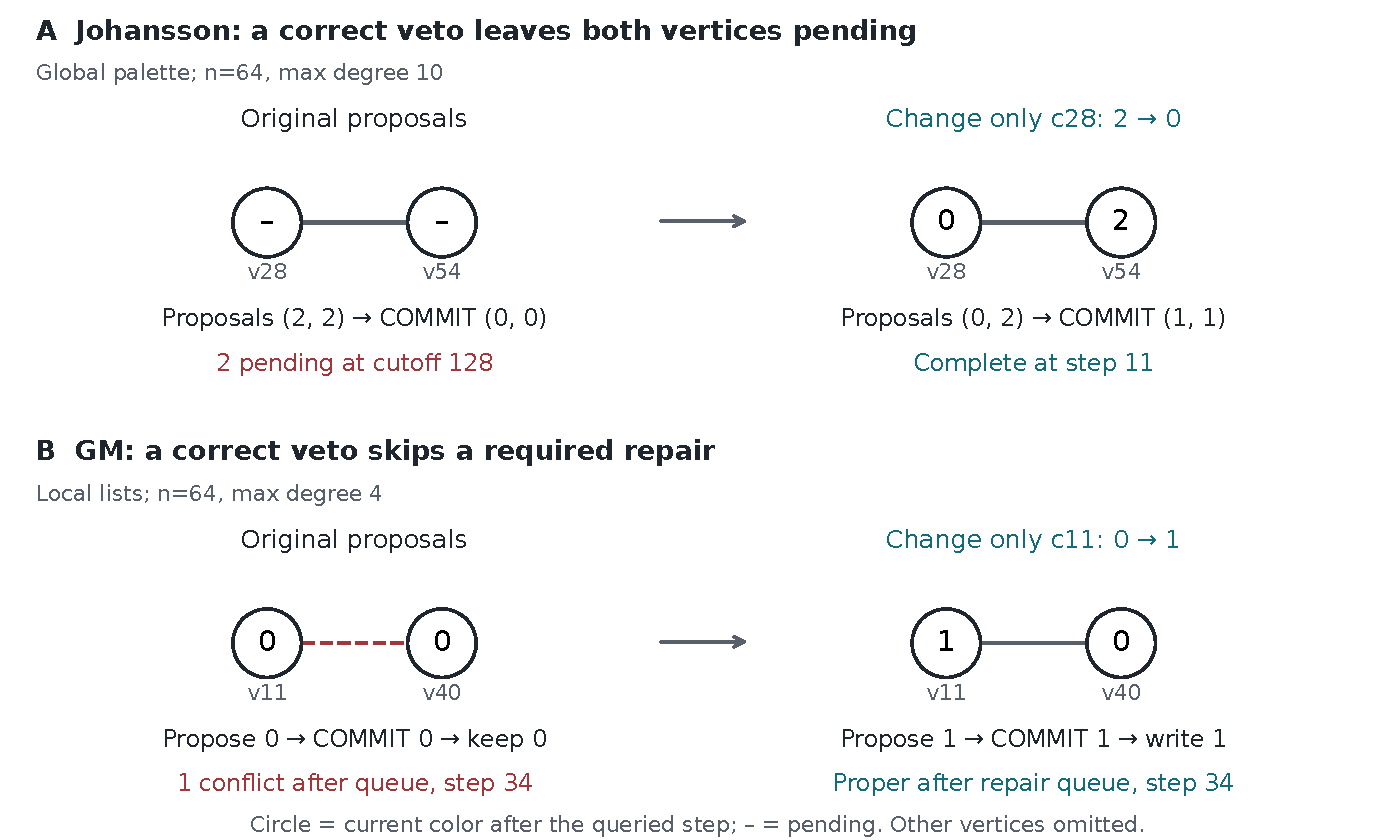
\includegraphics[width=\linewidth]{figures/revision-failure-mechanisms.pdf}
\caption{Two selected copied witness executions, showing local fragments
after one queried application. A: Johansson steps 10 to 11, with free colors
$\{0,2\}$ at both vertices. B: GM steps 32 to 33, with list $\{0,1\}$ at
the scheduled vertex 11; the dashed edge is an existing conflict. Changing
one proposal and recomputing learned COMMIT completes each copied run.
Exact-COMMIT substitution on unchanged proposals preserves both failures.
All other messages and first-stage tensors stay fixed at the intervention;
these cases do not estimate a population rescue rate. Full outcomes are
in Table~\ref{tab:rescues}.}
\label{fig:failure-mechanisms}
\end{figure}


These controls separate a proposal defect from an incorrect veto in the
selected states. Exact-COMMIT substitution is an identity at these already
correct vetoes, not an all-state oracle replacement or an audit of COMMIT
everywhere. The controls do not establish that changing the proposal module
would fix every failed execution, or that the first latent calibration
discrepancy caused the observed terminal failure.


Eleven other failed cells involve three matched E1 CT checkpoints, including
degree-three failures and incorrect simultaneous confirmations. Higher degree
cannot explain all of them. Alpha-threshold discrepancies are latent
calibration diagnostics, not supervised availability errors or causes by
themselves. The first temporal discrepancy is not automatically sufficient
to explain a final failure. Appendix~\ref{app:failures} lists every cell.

\paragraph{Exploratory scope.}
The separate pilot has 3,526/3,570 successes: two collisions, 42 CT resource
cutoffs. It spans regular $n=256$, degrees 2,3,4,5,10,20,50,100,200, sizes
through 1,024 at degree 3 or 10, plus heterogeneous/local cases. A ten-second
cap was applied only to unfinished dense CT cells after some longer degree-50
successes existed. These unequal resource horizons do not permit homogeneous
success-rate ranking. One run per checkpoint/cell is exploratory.
The later size pilot gives 240/240 for sixty Luby/Johansson/CT/JP checkpoints
on regular $n=2048,4096$, degrees 3,10, one run per point. It contains four
labeled graphs and twenty tapes, separately from confirmation. GM/Greedy
size pilots stop at 1,024; BE stays outside this extension.
Confirmation therefore reaches degree ten at size 64, and size 256 at degree
four, not their full cross-product, degree 200, or size 4,096.

\paragraph{Scale witness and confounding.}
Degree changes global $K$ and CT preferences simultaneously. A posthoc typed
probe keeps an edge endpoint's degree one and local list $\{0,1\}$ fixed,
while a separate star raises global $\Delta$. Preferences $\Delta$ and
$\Delta-1$ make it the strict color-zero winner. All fifteen primary CF CT
policies reject its queried COMMIT from degree ten in the main embedding.
Legacy preference/3 units alter responses but do not fix all tested cases.
Both encodings preserve order. This is scale sensitivity of fixed policies,
not an information obstruction, a demonstrated rounding cause or a random
functional failure rate. No degree-only causal effect independent of $K$
and private-input scale is identified.

\section{What Confirmation Can and Cannot Guarantee}\label{sec:interpretation}
Safety and progress require different hypotheses. Exact availability and
equal-offer rejection preserve partial properness; always waiting is also
safe. For independent fresh proposal laws $q_v$ and participation $p_v$,
conditioned on history before those draws, the exact anonymous rule gives
\[
 \Pr(v\text{ commits}\mid S)=p_v\sum_{c\in\A_v}q_v(c)
 \prod_{u\in U_v}(1-p_uq_u(c)).
\]
Uniform available proposals yield the exact teachers' positive progress
bounds (Appendix~\ref{app:teachers}). Concentrating both endpoint proposals
on the same color can make the product zero under always-active Johansson,
even with perfect COMMIT. A finite draw probe demonstrates observed
concentration, not a proof of zero alternative probability.

GM uses a different argument: exact marks cover all speculative conflict
edges and every queued repair writes a currently free color. The queue
visits each marked vertex once. Correctly rejecting an occupied proposal
satisfies the continuation rule but violates the required repair-write
condition; there is no automatic retry. The two witness interventions test
these specific missing hypotheses directly.

The finite-type MAX condition in Appendix~\ref{app:math} certifies one
canonical COMMIT predicate when every required local type satisfies the
sign inequalities. It does not certify candidate diversity, scheduled
repair, or palette-context invariance. All 45 selected canonical transfer
cores fail that sufficient condition; five \emph{different} historical E1
weights pass conditional certificates. Successful finite runs do not convert
either cohort into a universally certified learned algorithm. The elementary
ID-observation obstruction and representation controls appear in
Appendix~\ref{app:ids}; numerical sensitivity is distinguished from missing
information.


\section{Discussion and Limits}
Continuation tests identify behavior under a declared extension of a rule;
they do not establish that the native trace uniquely specifies that extension.
The historical BE comparison shows a procedure difference under unequal
budgets and reused development queries. The new experiment isolates an
acquisition-strategy contrast at equal target and conditioning budgets on
held-out sufficient input types. The class/support audit changes its
interpretation: native GM color confirmations are all positive, and the
BE occurrence-level metric rewards an eligibility rule that ignores occupancy.
CF's stronger BE type accuracy coexists with false negatives and fewer
autonomous successes. Nearly all test oracle configurations already occur in
CF training. Neither new-condition extrapolation nor an advantage over other
informative-negative acquisition strategies is established.
Paired first-stage tensors, reused states and graph/tape sharing
are recorded rather than counted as independent training replications.

Correct confirmation and autonomous completion are distinct outcomes. The
rescues demonstrate sufficiency of a candidate change in two selected
witnesses, not a population-wide remedy or a deployable oracle-assisted policy.
The selected new BE diagnoses distinguish COMMIT generalization failures
despite acquired-label fit from an upstream participation omission with a
correct conditional COMMIT response. The latter is localized in one original
run; a local participation query does not establish a complete-run rescue.
Degree transfer also changes palettes and, for ColorTrials, preference scale;
the posthoc scale probe does not identify a degree-only effect. Pilot and
confirmatory domains differ; size 4,096 and degree 200 are exploratory limits
at different coordinates, not a jointly tested operating region.

The supplied schedules, algebraic predicates and decoding delimit the learned
algorithm. Ideal-randomness proofs require explicit conditions not established
uniformly for these networks. All-pass native packages use heterogeneous
protocols (Appendix~\ref{app:coverage}), and no architecture ranking follows.
Output-law studies concern complete vectors/status, not just properness or
one-node marginals; nonrejection is not equality (Appendix~\ref{app:laws}).
The forty original Pedro weights are available in this workspace and match
their inventory hashes; this corrects the earlier local-availability statement
but does not constitute a new replay of that cohort. The later closure archive
and its 810,000 raw student rows remain unavailable here. Its reported totals
are retained with source provenance, not presented as independently regenerated.
Independent scientific review of this revision remains pending.

\section{Conclusion}
Perfect measured native agreement can coexist with wrong continuation
responses. Auditing the target contract, class balance and local input types
makes that gap interpretable. A separate prospective comparison addresses a
narrower equal-budget question. Its gains must be interpreted against label
coverage, the programmed diagnostic and the limited novelty of held-out
contexts. In BE, improved type accuracy does not prevent worse autonomous
completion. Frozen failures and component interventions
show why correct rejection alone does not supply proposal diversity or a
required scheduled repair. These distinctions provide testable explanations
of learned local behavior while keeping finite evidence separate from
universal guarantees.

\appendix
\section{New Prospective Replicas and Costs}\label{app:prospective}

\begin{longtable}{llrrrrr}
\caption{All new final seed outcomes. BA is a percentage; differences are
percentage points. Successes are out of 1,000 per model. N expands native confirmations.}\\
\toprule Teacher & Seed & N BA & CF BA & Difference & N success & CF success \\
\midrule\endfirsthead
\toprule Teacher & Seed & N BA & CF BA & Difference & N success & CF success \\
\midrule\endhead
BE & 105001 & 99.435 & 52.756 & -46.679 & 1000 & 100 \\
BE & 105002 & 99.334 & 99.872 & +0.538 & 1000 & 1000 \\
BE & 105003 & 99.539 & 99.987 & +0.448 & 1000 & 1000 \\
BE & 105004 & 50.193 & 99.923 & +49.730 & 1000 & 1000 \\
BE & 105005 & 50.320 & 99.885 & +49.565 & 1000 & 1000 \\
BE & 105006 & 99.152 & 99.897 & +0.746 & 1000 & 1000 \\
BE & 105007 & 50.348 & 99.923 & +49.575 & 1000 & 1000 \\
BE & 105008 & 99.195 & 52.094 & -47.101 & 1000 & 101 \\
BE & 105009 & 99.462 & 99.859 & +0.397 & 1000 & 1000 \\
BE & 105010 & 99.451 & 99.949 & +0.498 & 204 & 204 \\
GM & 105001 & 50.000 & 100.000 & +50.000 & 1000 & 1000 \\
GM & 105002 & 50.000 & 100.000 & +50.000 & 1000 & 1000 \\
GM & 105003 & 50.000 & 100.000 & +50.000 & 1000 & 1000 \\
GM & 105004 & 50.000 & 100.000 & +50.000 & 1000 & 1000 \\
GM & 105005 & 50.000 & 100.000 & +50.000 & 1000 & 1000 \\
GM & 105006 & 50.000 & 100.000 & +50.000 & 1000 & 1000 \\
GM & 105007 & 50.000 & 100.000 & +50.000 & 1000 & 1000 \\
GM & 105008 & 50.000 & 100.000 & +50.000 & 1000 & 1000 \\
GM & 105009 & 50.000 & 100.000 & +50.000 & 1000 & 1000 \\
GM & 105010 & 50.000 & 100.000 & +50.000 & 1000 & 1000 \\
\bottomrule
\end{longtable}


\begin{table}[htbp]\centering\small
\begin{tabular}{llr}
\toprule Teacher & Base target component & Count range across ten banks \\
\midrule
BE & confirmation & 944--944 \\
BE & linial point & 168--168 \\
BE & participation & 944--944 \\
BE & proposal & 944--944 \\
GM & confirmation & 744--754 \\
GM & conflict mark & 738--768 \\
GM & participation & 744--754 \\
GM & proposal & 744--754 \\
\bottomrule
\end{tabular}
\caption{Base supervision sums to exactly 3,000 per seed. Both arms add
3,600 auxiliary COMMIT targets. Context values and simulator costs are
reported separately, not absorbed into a free-label assumption.}
\end{table}

Each pair physically acquires 10,200 optimization targets: one shared
3,000-target base and two 3,600-target auxiliary banks. Each model accesses
6,600 targets, so shared physical acquisition and summed model access differ.
The shared auxiliary P/C context contains 7,200 root scalar occurrences and
additional real-neighbor occurrences. Base root P/C context overlaps base
target labels; its neighbor conditioning values are also recorded separately.
These are scalar occurrences, not claims about distinct simulator calls.

\code{results/paper-revision-20261030/prospective-summary.json} records the
per-seed component counts, complete-query duplicates, phase quotas, contexts
considered/rejected, observed simulator states, acquisition CPU/wall time and
paired bootstrap outputs. Training records separately retain presentations,
visited targets, source/data hashes and optimizer CPU/wall time. One run's
wall time includes a shared-host memory stall; wall time is not a FLOP or
teacher-sample-efficiency estimate. All training remains at update 1,500.
The original source/config freeze predates scientific training; the complete
forty-weight freeze is dated 30 October 2026, 10:11:58 UTC, before any new
final diagnostic generation. No final outcome selects a milestone, protocol
change, seed exclusion or replacement model.

The recorded source freeze covers the enumerated files, not a complete
transitive dependency or environment lock. In particular, graph generation,
storage and sample-complexity data helpers outside that list are not sealed
by this receipt. Their stability is not independently timestamped here.
The original freeze is preserved; this limitation is not repaired by
retrospectively adding hashes to it.

\subsection{Prospective acquisition and sufficient key}\label{app:prospective-method}
This specifies the already executed acquisition, not a revised protocol.
Color queries use four option indices, $q=c_v\in\{0,1,2,3\}$, degree at
most three, and legal teacher-prefix states. Auxiliary and diagnostic graph
streams use separate namespaces; their sizes are respectively 8/12/16/24
and 28/36. The frozen configuration and graph generators identify the streams.

For each queried color, let $w_j$ be permission and $u_j$ the supplied
pending-or-permitted bit in GM. In BE the queried-stage adapter sets $u_j=1$.
Let $b_j$ be the current-own-color indicator for $q$ in GM and zero in BE.
Let $o_{vj}$ be the neighbor's occupancy of the receiver's queried KW option
in BE and $b_j$ in GM. Set $\kappa_v=\operatorname{sgn}(a_v-q_{\rm KW})$
in KW, where $q_{\rm KW}=\lceil4B/5\rceil$, and zero in GM. Here $a_v$
is the auxiliary color; it is distinct from the queried option index $q$.
GM also supplies $\sigma_{vj}=\operatorname{sgn}(ID_j-ID_v)$ and the
same-slot indicator $\tau_{vj}$; both are zero in BE's queried-stage adapter.
With the actual supplied messages $p_j,c_j$, define
\[
 r_v=(u_v,b_v,p_v,\mathbf1[u_v>1/2]),\qquad
 m_{vj}=(u_j,o_{vj},p_j,\mathbf1[u_j>1/2\ \land\ c_j=q],
             \sigma_{vj},\tau_{vj}),
\]
\[
 K=(T,\phi,w_v,\kappa_v,r_v,
       \operatorname{sort}\{m_{vj}:j\in N(v)\}).
\]
The neighbor collection is a set: identical message types occur once.
This is sufficient for the fixed-weight queried-slot MAX computation, not a
minimal oracle quotient, a proposal key or a classifier of LINIAL/DETECT.
The original code represents the BE offset as the signed encoded offset;
its sign is exactly $\operatorname{sgn}(a_v-q_{\rm KW})$.

For the hash, all bits are integers 0/1 and signs are $-1,0,1$; $T$ is the
string \code{BE_BASE_D3} or \code{SPECULATIVE_GM}. The phase integer $\phi$
is 5 for KW, 1 for ASSIGN and 3 for REPAIR. Tuples/sets are serialized as
JSON lists, with neighbor tuples in lexicographic order and separators
\code{,} and \code{:} with no spaces. Prefix the UTF-8 JSON by the literal
salt \code{revision-20261030-commit-types-v1}, with no separator. Interpret
the first eight SHA256 bytes as a big-endian unsigned integer. Residue zero
modulo five denotes held-out types. This reserves 20\% of hash buckets;
it need not reserve exactly 20\% of observed types or occurrences.

Acquisition proceeds as follows.
\begin{enumerate}
\item Retain native base targets until the 3,000-component budget is filled.
Color-phase base queries must have training keys; LINIAL/DETECT use their
separate native targets and do not receive this COMMIT filter.
\item In each auxiliary color-phase batch with an unfilled quota, enumerate candidate roots with
a running cursor $i$ before any filtering. Set $k=i\bmod4$ and
$c'_v=(c_v+k)\bmod4$. Draw an independent uniform value for every considered
root. Set $p'_v=w_v$, except that $k=3$ and a draw below 1/4 set $p'_v=0$.
All real-neighbor P/C values stay native.
Advance the cursor for all considered roots, including rejected roots.
\item Training retains a root only when both $K(S,p,c)$ and $K(S,p',c')$
are training types, subject to the 3,600 KW or 1,800 ASSIGN/1,800 REPAIR
quotas. Compute its labels only after this filter. The native arm receives
one native confirmation and CF one intervened confirmation on the same state.
\item After freezing all forty models, the diagnostic stream applies the
same intervention, but retains a root if its intervened key is held out.
The native key is unrestricted at test. Retain exactly 4,000 KW or 2,000
ASSIGN/2,000 REPAIR queries per seed, without filtering on truth labels.
\end{enumerate}
The intervention RNG is seeded by the frozen namespace, teacher, training
seed, acquisition kind and the literal \code{intervention}. Native graph/tape
streams have their separate base/auxiliary/diagnostic suffixes. Filtering can
change offset and silence frequencies; the pre-filter silence probability is
not a claim about the retained distribution. No phase quota balances the
positive and negative truth labels within that phase.

\subsection{Post-test coverage and confusion audit}\label{app:prospective-audit}
All tables here are descriptive additions after the final test. Labels are
recomputed from raw encoded state arrays and agree with stored base, auxiliary
and final color confirmations. Fine keys are reconstructed from those arrays;
their training/test unions equal the delivered key files and obey the original
hash filter. Model predictions are summarized from frozen result records;
this audit does not rerun neural inference or train another model.
{\small

\begin{longtable}{lllrr}
\caption{Ranges over ten seeds of base plus auxiliary color-COMMIT targets.
LINIAL and DETECT have different targets and are excluded. Minima and maxima
in separate columns need not occur at the same seed.}\\
\toprule Teacher & Phase & Arm & Positive labels & Negative labels \\
\midrule\endfirsthead
\toprule Teacher & Phase & Arm & Positive labels & Negative labels \\
\midrule\endhead
BE & KW & native & 152--189 & 4,355--4,392 \\
BE & KW & cf & 113--147 & 4,397--4,431 \\
GM & ASSIGN & native & 2,417--2,440 & 0 \\
GM & ASSIGN & cf & 2,108--2,153 & 277--326 \\
GM & REPAIR & native & 1,904--1,932 & 0 \\
GM & REPAIR & cf & 1,119--1,171 & 749--793 \\
\bottomrule
\end{longtable}

}


\begin{longtable}{llrrrrr}
\caption{Final support and programmed diagnostic by seed. Types are distinct
fine sufficient keys; mass is the largest key's fraction of 4,000 queries.
Overlap is the fraction of occurrences whose coarser oracle configuration was
seen by CF training. Mass, overlap, BA and type accuracy are percentages.}\\
\toprule Rule & Seed & Types & Max mass & Overlap & Gate BA & Gate type acc. \\
\midrule\endfirsthead
\toprule Rule & Seed & Types & Max mass & Overlap & Gate BA & Gate type acc. \\
\midrule\endhead
BE & 105001 & 20 & 95.38 & 99.750 & 99.679 & 80.000 \\
BE & 105002 & 23 & 96.03 & 99.475 & 99.770 & 78.261 \\
BE & 105003 & 17 & 96.30 & 99.825 & 99.770 & 82.353 \\
BE & 105004 & 20 & 95.17 & 99.750 & 99.614 & 80.000 \\
BE & 105005 & 18 & 95.62 & 100.000 & 99.731 & 83.333 \\
BE & 105006 & 20 & 95.05 & 99.800 & 99.589 & 80.000 \\
BE & 105007 & 21 & 95.15 & 99.725 & 99.704 & 80.952 \\
BE & 105008 & 20 & 95.53 & 100.000 & 99.706 & 85.000 \\
BE & 105009 & 22 & 95.67 & 99.725 & 99.756 & 86.364 \\
BE & 105010 & 17 & 96.23 & 99.775 & 99.757 & 76.471 \\
GM & 105001 & 89 & 23.80 & 100.000 & 53.055 & 61.798 \\
GM & 105002 & 84 & 23.62 & 100.000 & 52.910 & 63.095 \\
GM & 105003 & 92 & 23.82 & 100.000 & 53.204 & 63.043 \\
GM & 105004 & 86 & 24.60 & 100.000 & 53.182 & 62.791 \\
GM & 105005 & 91 & 23.88 & 100.000 & 52.686 & 63.736 \\
GM & 105006 & 83 & 24.10 & 100.000 & 52.921 & 60.241 \\
GM & 105007 & 86 & 24.52 & 100.000 & 53.193 & 62.791 \\
GM & 105008 & 87 & 23.85 & 100.000 & 53.111 & 60.920 \\
GM & 105009 & 89 & 23.80 & 100.000 & 53.065 & 64.045 \\
GM & 105010 & 82 & 24.60 & 100.000 & 53.005 & 60.976 \\
\bottomrule
\end{longtable}


{\small

\begin{longtable}{lllrrrr}
\caption{Confusion counts summed over ten final banks, 40,000 queries per
teacher/procedure. Within eligible active queries, positives are free options
and negatives occupied options. Silent and ineligible queries are negative.
No GM query is ineligible. These are accounting totals, not IID replications.}\\
\toprule Rule & Stratum & Procedure & TP & TN & FP & FN \\
\midrule\endfirsthead
\toprule Rule & Stratum & Procedure & TP & TN & FP & FN \\
\midrule\endhead
BE & eligible active & native & 995 & 0 & 228 & 0 \\
BE & eligible active & cf & 814 & 228 & 0 & 181 \\
BE & eligible active & gate & 995 & 0 & 228 & 0 \\
BE & eligible silent & native & 0 & 91 & 42 & 0 \\
BE & eligible silent & cf & 0 & 52 & 81 & 0 \\
BE & eligible silent & gate & 0 & 133 & 0 & 0 \\
BE & ineligible & native & 0 & 26,956 & 11,688 & 0 \\
BE & ineligible & cf & 0 & 38,644 & 0 & 0 \\
BE & ineligible & gate & 0 & 38,644 & 0 & 0 \\
GM & eligible active & native & 15,554 & 0 & 22,963 & 0 \\
GM & eligible active & cf & 15,554 & 22,963 & 0 & 0 \\
GM & eligible active & gate & 15,554 & 0 & 22,963 & 0 \\
GM & eligible silent & native & 0 & 0 & 1,483 & 0 \\
GM & eligible silent & cf & 0 & 1,483 & 0 & 0 \\
GM & eligible silent & gate & 0 & 1,483 & 0 & 0 \\
\bottomrule
\end{longtable}

}
The reproducible analysis and input hashes are
\code{scripts/audit-revision-continuations.py} and
\code{results/paper-revision-20261030/continuation-audit.json}.

\subsection{Selected BE failure diagnoses after the test}\label{app:be-failure-diagnostics}
Frozen-model inference covers both arms of BE seeds 105001, 105002, 105004,
105008 and 105010, plus both GM arms in 105001. This deliberately selected
set includes good and bad outcomes; it does not estimate their prevalence.
There are 102,128 COMMIT predictions on existing native-color,
auxiliary-training and final banks. All 48,000 final predictions
reproduce the original confusion counts; no weights, split or primary
results are changed. This diagnosis uses neural inference, separately from
the preceding array-only coverage audit.


\begin{table}[htbp]\centering\small
\begin{tabular}{lrrrrr}
\toprule CF seed & Aux. BA & Final BA & Aux. FN & Final FN & Final FP \\
\midrule
105001 & 99.510 & 52.756 & 1 & 98 & 10 \\
105008 & 100.000 & 52.094 & 0 & 83 & 16 \\
\bottomrule
\end{tabular}
\caption{Selected BE COMMIT generalization failures. BA is a percentage.
Each row evaluates the arm's 3,600 acquired auxiliary queries and the 4,000
held-out final queries. All auxiliary targets were visited during training;
neither selected model has an auxiliary false positive. The contexts differ,
so this is a descriptive fit/test contrast, not a new randomized comparison.}
\label{tab:be-fit-test}
\end{table}

The two CF models also classify all 944 native-color base queries correctly.
Their held-out-context errors coexist with near-perfect acquired-label fit;
this does not identify a unique shortcut, optimization cause or limitation
of representational capacity.

For seed 105010, native and CF first-stage tensors are identical. On 4,000
teacher-prefix test states their participation head omits 13 of
118 eligible roots, with no false activation. On 3,600 auxiliary
states it omits 4 of 128 eligible roots and falsely activates
1 ineligible root. Auxiliary P/C values condition the COMMIT loss;
they are not direct participation-loss targets. These first-stage scores on
auxiliary states are evaluations, not evidence of failure to fit a
participation training objective there. Candidate options equal the native
ones throughout both banks, with no occupied proposals at eligible roots.

The witness is \code{final-s105010-0000}, a 32-node path in the native arm.
Replay preserves the first 32 original cases in their original order,
cohort size 32 and root batch size 1,024. All 32 terminal color vectors,
step counts, failures, invariant flags and correctness flags match the
original records. In the selected case the state before step 7 is a
proper auxiliary coloring bounded by 21. Vertex 31 has value 17
and must recolor when the interpreter lowers the bound to 17.
Its participation logit is -0.420059, so it waits, leaving 17 outside
$[0,17)$. Its option 0 decodes to the free value 12,
also chosen by the exact native rule. The actual COMMIT logit -11.225789
correctly rejects silence. Setting only this root's participation bit to
true, with identical first-stage tensors, candidates and all other messages,
gives logit +4.629150 and the correct positive oracle label. The
observer's re-evaluated actions match the original actions at this frame.
The intervention is only a local query; unchanged actions drive the replay.
It locates the first violation in this case, without showing that all 796
failed runs share this mechanism or that the intervened run would complete.

\path{scripts/probe-revision-be-failures.py} reproduces the diagnosis;
\path{results/paper-revision-20261030/be-failure-diagnostics.json} records
input hashes, counts, graph/tape seeds and the local intervention. This is
post-test explanatory evidence, not independent scientific review.


\section{Native Functional Coverage}\label{app:coverage}
The native result is \textbf{21/21 combinations under their respective
protocols}: five selected checkpoints per combination, each with 1,000/1,000
proper complete invariant-valid executions. Twelve (Luby, Johansson, JP,
Greedy across three cores) are historical passive packages, seeds
83101--83105. Nine (ColorTrials, BE, GM across three cores) are new CF
packages, seeds 94101--94105. The representative BE/CT weights use 4,000
updates and GM 500. Matched controls also close all nine; CF is not shown
necessary for native functional success.

\begin{table}[htbp]\centering\small
\begin{tabular}{lccc}
\toprule Teacher & E1 & DeepSets & Transformer \\
\midrule
Luby & H: 5/5 & H: 5/5 & H: 5/5 \\
Johansson & H: 5/5 & H: 5/5 & H: 5/5 \\
ColorTrials & N: 5/5 & N: 5/5 & N: 5/5 \\
JP & H: 5/5 & H: 5/5 & H: 5/5 \\
BE base & N: 5/5 & N: 5/5 & N: 5/5 \\
GM & N: 5/5 & N: 5/5 & N: 5/5 \\
Greedy & H: 5/5 & H: 5/5 & H: 5/5 \\
\bottomrule
\end{tabular}
\caption{Native coverage: each passing checkpoint has 1,000/1,000 successes.
H: historical passive; N: new CF. These protocols do not form a homogeneous
architecture-ranking experiment.}
\label{tab:coverage}
\end{table}

Final tests use sizes 32, 48, 64; family weights differ: seven historical
strata versus ten new strata of 100 runs. The 105 selected policies account
for 105,000 successful observations, not a success probability of an average
policy. Five training seeds are the treatment replication units.
Under independent Bernoulli trials with a common probability, 1,000/1,000
gives pointwise two-sided 95\% Clopper--Pearson lower limit
$0.025^{1/1000}=0.996318$; the one-sided limit is
$0.05^{1/1000}=0.997009$. For fixed independent nonidentical strata, AM--GM
makes the zero-failure formula conservative for the weighted average, not
each stratum. No simultaneous all-policy guarantee or universal correctness
follows. A selected successful budget is not a theoretical minimum.
The run-level interpretation also assumes semantically neutral batching.
Real-arithmetic message separation supports that premise; universal numerical
neutrality across floating-point batch contexts has not been certified.

\paragraph{Preserved negative results.}
The historical study's nine noncertifications under 500 updates are not
impossibility results. The pre-revision native-certification study retains
21 failed executions among
195,000 final observations across 39 packages and 170 distinct checkpoints;
some weights receive new batteries. All failures remain separate from the
selected all-pass set. Independent fixed-bank E1 controls compare 500 versus
1,500 updates along the same seed/checkpoint lineage, holding labels fixed
and using fresh final tapes. This is a more narrowly identified optimizer
contrast than matched versus CF; it does not establish a CF effect or
monotone benefit from more updates (Appendix~\ref{app:training}).

\section{Information and Identifiers}\label{app:ids}
Consider an initial two-node JP graph with identical anonymous observations
and fixed private inputs. Swapping the distinct IDs changes the required
root action from write to wait without changing the anonymous observation.
\begin{proposition}[Observation indistinguishability]\label{prop:ids}
If two admissible contexts have the same observation and different
deterministic target actions, no deterministic function of that observation
is correct on both. A randomized function cannot be almost surely correct
on both.
\end{proposition}
\begin{proof}
Equal inputs give equal outputs or equal conditional output laws. Different
point-mass targets cannot both be realized. For equiprobable binary contexts,
average correctness is at most $1/2$.
\end{proof}
This elementary interface obstruction is not a new distributed lower bound.
It requires indistinguishability, not numerical closeness, and does not
preclude solving coloring by a different rule. Historical integrated JP/GM
already had numeric ID differences; their failures were not ID blindness.

\begin{table}[htbp]\centering\small
\begin{tabular}{lrrrrr}
\toprule JP representation & 94101 & 94102 & 94103 & 94104 & 94105 \\
\midrule
\closureinput tables/closure-jp.tex
\bottomrule
\end{tabular}
\caption{Exploratory E1 JP control: same dimensions, initialization, 3,000
labels and 500 updates. Entries are development successes out of 60,
not final 1,000-run certifications.}
\label{tab:ids}
\end{table}
Relative comparisons achieve 60/60 in all five seeds. This supports
representation sensitivity under this budget. Numeric IDs/differences retain
order information, so finite failures do not prove inability to learn it.
Signs remove the need to resolve gaps as small as $1/65536$; they must arise
from one coherent order. BE uses actual ID arithmetic: increasing numeric
transformations need not preserve its polynomial trajectory.

\section{Exact Rules and Conditional Guarantees}\label{app:teachers}
Assume finite simple graphs, proper partial states where required, declared
lists of size at least $d(v)+1$, coherent observations and the specified
synchronous exchanges/schedules. Code domain guards and independent scalar
tests complement these arguments.
\begin{lemma}[Availability]
For a pending vertex, $|\A_v|\ge |C_v|-(d(v)-d_U(v))\ge d_U(v)+1$.
\end{lemma}
\begin{proof}
At most one distinct color per fixed neighbor is forbidden. Counting
duplicates only weakens the bound; differing local lists cause no problem.
\end{proof}
\paragraph{Luby/Johansson.}
Proposals avoid fixed colors, and exact equal-active-offer rejection prevents
simultaneous collisions. Permanent colors persist, giving safety by induction.
Condition on history/state before new private inputs, not a snapshot already
containing those inputs. If $q_v(c)$ is the proposal law, $p_v$ its independent
participation, with independent pairs across nodes, then
\begin{equation}\label{eq:progress}
\Pr(v\text{ commits}\mid S)=p_v\sum_{c\in\A_v}q_v(c)
\prod_{u\in U_v}(1-p_uq_u(c)).
\end{equation}
For uniform proposals and $p_u=1/2$, the chord bound
$\log(1-x)\ge-2\log(2)x$ on $[0,1/2]$ and Jensen yield
$\frac12 2^{-d_U(v)/|\A_v|}\ge1/4$.
For always-active Johansson, each pending neighbor of $v$ has at least two
free colors, so $q_u(c)\le1/2$. The same argument yields
$2^{-2d_U(v)/|\A_v|}\ge1/4$. These prove the specified variants' bounds;
they do not import a different algorithm's theorem
\citep{luby1993randomness,johansson1999coloring}.

\paragraph{ColorTrials.}
Let $D\ge\Delta$ be the common preference bound: $D=3$ natively, even on
lower-degree graphs, and $D=\Delta$ in the extension. Pending nodes draw
independent preferences for each color in $\{0,\ldots,D\}$. Only pending
neighbors for which the color is
available compete. The minimum strictly winning available color is chosen;
otherwise wait. Adjacent vertices cannot both strictly win one color.
For any $c\in\A_v$, the event of preference $D$ at $v$ and smaller
preferences at all at most $\Delta$ competitors has probability at least
$\rho_{\rm CT}=(D+1)^{-1}(D/(D+1))^\Delta>0$ for $D>0$.
It guarantees some write at $v$, perhaps a lower winning color. Isolates at
$\Delta=0$ finish in one step. The common global preference alphabet matters;
different local alphabets need another analysis. This is a repeated
subroutine inspired by symmetry breaking \citep{schneider2010symmetry}, not
a full multi-phase complexity claim.

\paragraph{Random termination.}
If each pending vertex has conditional progress at least $\rho>0$ at every
reachable state, iterated conditioning gives
$\Pr(T_v>t)\le(1-\rho)^t$ and
$\Pr(T>t)\le\min\{1,n(1-\rho)^t\}$. Thus ideal exact rules terminate
almost surely. Transfer uses at least 128 steps, enlarged for CT until this
ideal tail bound is at most $10^{-9}$. Neither arbitrary learned policies
nor finite PRNG orbits inherit the result automatically.

\paragraph{JP and Greedy.}
JP's pending strict maxima of coherent distinct IDs form an independent set.
First-fit exists by availability, and the remaining global maximum writes
each step, giving safety and at most $n$ steps. This synchronous variant is
inspired by \citet{jones1993parallel}. Greedy permits exactly one vertex in
increasing-ID order per step; first-fit avoids prior colors and completes in
$n$ writes. Global scheduling cost is supplied, not a free LOCAL operation.

\paragraph{Speculative GM.}
Split increasing-ID order into $\min(4,n)$ balanced blocks. ASSIGN visits
one position per block simultaneously. A later assignment avoids all earlier
neighbor colors, so only equal-slot vertices can conflict. DETECT marks the
smaller-ID endpoint of each equal-color/equal-slot edge. Every conflict is
covered; the unmarked subgraph is proper. Serial repair visits marked vertices
once in increasing-ID order and avoids all current neighbor colors. The last
repaired endpoint of any edge avoids the other; edges with no repaired
endpoint were already proper. Correctness follows in
$2\lceil n/\min(4,n)\rceil+m$ steps, $m\le n$. Every scheduled write/mark
must be correct. Missed learned repairs are not retried. This is the
implemented four-block variant \citep{gebremedhin2000scalable}, including
supplied barriers/queue, not a guarantee for arbitrary learned marks.

\paragraph{BE degree-three base case.}
Distinct IDs are initial proper auxiliary colors. Degree-at-most-four
polynomials over $\mathbb F_{13}$ encode them. A different neighboring
polynomial agrees at at most four points, so three neighbors block at most
twelve and $13>3\cdot4$ leaves a point. Encode selected point/value below
$13^2=169$. A second degree-at-most-two reduction over $\mathbb F_7$ has
a point because $7>3\cdot2$, yielding bound 49. Different chosen points
give different pairs; equal points have different unblocked values, proving
properness \citep{linial1992locality}.
For bound $B>4$ set $q=\lceil4B/5\rceil$. Colors below $q$ remain; each
high old color owns a disjoint four-option block in $[0,q)$, possible since
$4(B-q)\le q$. Three neighbors forbid at most three options. High--high
neighbors have disjoint blocks; high--low collisions are excluded by free
options. The sequence
$49\to40\to32\to26\to21\to17\to14\to12\to10\to8\to7\to6\to5\to4$
has thirteen KW reductions \citep{kuhn2006complexity}. Decoding does not search
for a good point/option. This is only the degree-three base construction
associated with \citet{barenboim2008linear}, not the general recursion.
At degree four, $13>4\cdot4$ fails; changing constants changes the variant.

\section{Conditional Representation and Probability Results}\label{app:math}
The following elementary arguments are not claimed new general GNN-learning
theorems. Checkpoints satisfy their hypotheses only where verified.
\begin{proposition}[Diffuse proposals]
Assume a proper state, exact rejection, independent node-private draws,
independence of participation/candidate within nodes,
$0<p_{\min}\le p_v\le p_{\max}<1$, proposal support in $\A_v$, and
$\max_cq_v(c)\le\beta/|\A_v|$. Then
$\Pr(v\text{ commits}\mid S)\ge
p_v(1-p_{\max})^{\beta d_U(v)/|\A_v|}
\ge p_{\min}(1-p_{\max})^\beta$.
Only $v$ needs the concentration bound for this individual-node statement.
\end{proposition}
\begin{proof}
The log chord gives $\log(1-x)\ge ax$ for
$a=\log(1-p_{\max})/p_{\max}<0$, $0\le x\le p_{\max}$.
Write $\Lambda_c=\sum_{u\in U_v}p_uq_u(c)$.
Equation~\eqref{eq:progress} is at least
$p_v\sum_cq_v(c)e^{a\Lambda_c}\ge p_ve^{a\sum_cq_v(c)\Lambda_c}$ by Jensen.
The weighted load is at most $\beta p_{\max}d_U(v)/|\A_v|$; each neighbor
has mass at most one on $\A_v$. Multiplication by $a<0$ reverses that
inequality, and availability gives the last bound. Isolates use the empty
product.
\end{proof}
\begin{corollary}[Diffuse submass]
If the concentration bound holds only on $S_v\subseteq\A_v$ of mass
$\eta_v>0$, the lower bound is
$p_v\eta_v(1-p_{\max})^{\beta d_U(v)/(\eta_v|\A_v|)}$.
Uniform $\eta_v\ge\eta>0$ at every reachable state implies uniform progress
$p_{\min}\eta(1-p_{\max})^{\beta/\eta}$.
\end{corollary}
\begin{proof}
Drop nonnegative terms outside $S_v$, renormalize by $\eta_v$, and repeat.
$x b^{\beta/x}$ increases for $x>0$, $0<b<1$, since its derivative is
$b^{\beta/x}(1-\beta\log b/x)>0$.
\end{proof}
\begin{example}[Safety without useful progress]
On a $K$-clique with $K\ge2$ colors, deterministic color-zero proposals,
participation $1/2$ and exact rejection progress only with exactly one active
vertex: probability $K/2^K$, expected first-progress time $2^K/K$.
Always-active vertices never progress. A shared uniform candidate draw has
uniform individual marginals and the same slow law; independence in
\eqref{eq:progress} cannot be replaced by marginal uniformity.
\end{example}

\begin{proposition}[Canonical finite-type MAX COMMIT]\label{prop:max}
Assume legal canonical per-color inputs/gating, nonnegative shared second
messages, componentwise MAX with zero empty aggregate, and exact proposed-slot
gather. The pending active center's queried-slot vector is $(1,0,1,1)$;
neighbor vectors $(\text{pending},\text{owns}_c,\text{participates},\text{offers}_c)$
are among
\[
(0,0,0,0),(0,1,0,0),(1,0,0,0),(1,0,0,1),(1,0,1,0),(1,0,1,1).
\]
If all 64 type-subset COMMIT signs accept precisely subsets without the
fixed-color or active-equal-offer conflict types, the rule is exact at any
legal degree/palette in real arithmetic and preserves properness.
\end{proposition}
\begin{proof}
MAX is associative, commutative and idempotent; multiplicities disappear.
Nonnegative messages admit zero identity. Gathering the proposed slot
removes other slots. The 64 subsets therefore enumerate all aggregates.
Excluding the two conflict types prevents old/simultaneous collisions.
Induction gives safety, with no progress conclusion.
\end{proof}
This does not cover continuous preference or native residual contexts,
multiple offers, SUM or MEAN. Outward-rounded float64 intervals enclose
float32-stored weights as real coefficients. A separate mode adds
$\gamma_{m+2}$ float32 affine error and a subnormal allowance, conditional
on IEEE rounding, no overflow and no TF32/lower precision. It is not a proof
for arbitrary GPU kernels. Five historical E1 weights pass; all 45 selected
Luby/Johansson/Greedy transfer cores fail the sufficient all-types condition.
Failure of a sufficient certificate alone does not prove a reachable failure.

\begin{proposition}[MEAN dilution; SUM construction]
Fix degree/palette-independent messages $m_o,m_f$ and a continuous classifier
$F$ for a fixed active center. If $F(m_o)>0$, a MEAN interface accepts a
conflicting star with sufficiently many ordinary neighbors. A SUM interface
can represent exact conflict presence in real arithmetic.
\end{proposition}
\begin{proof}
A star with $d$ ordinary leaves and one fixed neighbor owning the candidate
has mean $(d m_o+m_f)/(d+1)\to m_o$. Continuity and strict acceptance imply
false acceptance at some finite $d$. If $F$ is $L$-Lipschitz, it suffices
that $d+1>L\|m_f-m_o\|_\infty/F(m_o)$. For SUM, use the legal-type conflict
bit $b=o+\operatorname{ReLU}(p+a-1)$ and head $1/2-\sum_ub_u$.
\end{proof}
The MEAN statement assumes no separate degree/palette input and says
nothing about reachability of the constructed state. SUM's observed failure
is not impossibility of representing this predicate.
An order-free equivariant slot scorer with identical available-slot inputs
and invariant pooled context gives tied scores for fixed private input;
it cannot select distinct ordered ranks without order features or external
tie-breaking. Main scorers have positions, so this obstruction does not
explain their errors automatically.

\section{Training, Certification and Historical Provenance}\label{app:training}
\begin{longtable}{lllrrrr}
\caption{Selected native packages: actual acquired labels per seed (ranges
where necessary), updates and total parameters. Every row has five policies
and 1,000/1,000 successes each. Historical seeds 83101--83105, new 94101--94105.}
\label{tab:native21}\\
\toprule Teacher & Core & Cohort & Labels & Updates & Parameters & Pass \\
\midrule\endfirsthead
\toprule Teacher & Core & Cohort & Labels & Updates & Parameters & Pass \\
\midrule\endhead
\closureinput tables/closure-native21.tex
\bottomrule
\end{longtable}
Historical sources are \code{results/sample-complexity/certification.json},
frozen candidates and raw final rows. New sources are
\code{results/multiteacher-counterfactual/plans/successful-policies.json}
and confirmation freezes/rows. Prefix budgets reuse labels and seeds; they
are not independent replications or theoretical sample-complexity scaling.
The new packages do not rewrite historical noncertifications as successes.

Source commits include Pedro audit \code{6836d855}, paper study
\code{b5427faf}, integration \code{a54a18e3}, sample complexity
\code{61f39760}, counterfactual \code{291d4b82}, degree \code{71153993}.
These are branches/worktrees in shared history, not independent copies of
every experiment. Old rows/protocols remain immutable; the previous manuscript
is archived under \code{paper/ucgnn/archive/pre-closure-71153993.tex/pdf}.

\paragraph{Optimizer controls and costs.}
Independent E1 confirmation compares 500/1,500 updates at nominal 3,000
native labels for Luby, JP and BE, five paired seeds and new final tapes.
Only optimizer effort differs along the same training lineage. Six arms and
all seed outcomes remain in
\code{results/sample-complexity/optimization-confirmation/results.json}.
It identifies additional-optimization effects for those bank/seed conditions,
not CF effects or optimal/monotone update counts.
Luby and JP complete 1,000/1,000 per seed at both milestones. BE moves from
72,90,84,92,42 successes per 1,000 to 1,000 in every seed; these are the
strongest resource-controlled optimizer results in the present evidence.
The small-width and no-communication baselines below share native prefixes,
500 updates and paired seed conventions with E1. They are development
controls, not optimized competitors or proof that every coloring rule needs
communication. No-communication erases received states, relations and masks
while retaining local inputs and external permissions. Small uses widths $8/4$.
\begin{table}[htbp]\centering\small
\begin{tabular}{llll}
\toprule Teacher & E1 & Small & No communication \\
\midrule
\closureinput tables/closure-baselines.tex
\bottomrule
\end{tabular}
\caption{Native development controls at nominal 3,000 labels and 500 updates.
Each entry lists successes out of 28 for seeds 83101--83105 individually.}
\end{table}
Dataset manifests record simulation steps, native/added labels, generation
CPU/wall time and bytes. In the historical CF acquisition, four labels per
color root are charged even if
queries coincide: these are conservative acquisition counts, not distinct
input counts. Checkpoints retain Adam, all RNG states, visitation and query
caches. The archived closure step itself trained no scientific models;
the separate forty-model prospective trial has its own training/freeze
receipts. Disposable technical gradient
tests produce no weights used in results. The evidence ledger identifies
all selected hashes and full label-generation costs.
\begin{table}[htbp]\centering\small
\begin{tabular}{lrrrr}
\toprule Teacher & Native labels & Added CF labels & Bank CPU seconds & Stored MB \\
\midrule
\closureinput tables/closure-label-cost.tex
\bottomrule
\end{tabular}
\caption{Acquisition cost of the complete shared native/CF bank, range over
five seeds. CPU time includes simulation, encoding and both label types;
it is not the isolated marginal CF cost. Decimal MB includes replay witnesses.
Training costs are separate.}
\end{table}

\section{Continuation Diagnostics and Dependence}\label{app:cf}
\begin{table}[htbp]\centering\small
\begin{tabular}{rrrrrrrr}
\toprule & \multicolumn{3}{c}{Correct / 99,840} & & \multicolumn{3}{c}{Unseen-type correct} \\
Seed & Passive & Matched & CF & Subset size & Passive & Matched & CF \\
\midrule
\closureinput tables/closure-be-seeds.tex
\bottomrule
\end{tabular}
\caption{Exact BE/E1 original numerators and posthoc novelty subsets.
Subset sizes count correlated query occurrences, not distinct types.}
\end{table}
The sufficient key comes from actual BE second-stage inputs, not its label.
Real centers have pending bit one and own-slot bits zero; ID/slot residuals
are zero. KW substitutes receiver-relative option equality for neighbor own
bits. QueryPolicy signs the offset. The root queried slot has offer bit one;
other slots vanish under gather. Each valid neighbor contributes occupied
query bit, participation and offer/query equality; MAX removes duplicates.
With phase, root permission, signed offset and root participation, this
determines the real queried-slot logit at fixed weights. It is not a
sufficient key for proposals. Train keys include native and all stored CF
queries. There are 58--65 distinct training keys and 115--132 diagnostic keys
per seed, with highly unequal occurrence counts. Complete serialized input
hashes retain irrelevant fields and measure a different novelty notion.

The diagnostic reconstruction is \code{scripts/final-counterfactual-audit.py}.
It reuses the original queries/RNG, reproduces all numerators, and records
each checkpoint and bank hash. Stored label checks find zero inconsistencies;
they validate the stated oracle, not graph-wide realizability of every query.
We use five paired seed ranges, not decision-level significance. Even five
same-sign pairs give exact two-sided sign-test $p=2/2^5=0.0625$ under an
exchangeable-sign null, before multiplicity. Shared BE/GM heads and repeated
states cannot increase the independent training sample size.
Positive counts across seeds are 3,070,2,895,2,891,2,773,3,115;
full confusion/eligibility strata are in
\code{results/final-closure/review-ml-be-strata.json}.
For unseen-type subsets positives are 52,108,90,56,60 and negatives
497,351,627,466,662. All arms have zero false negatives. The distinction
concerns rejecting negative continuations under the explicitly chosen
oracle; native traces alone do not uniquely specify off-policy semantics.

\section{Failure Inventory and Statistical Units}\label{app:failures}
The complete table is \code{results/final-closure/generalization-cells.csv}.
The factor table separates teacher, architecture, checkpoint, seed, size,
degree, palette, family and cohort within stage. The following lists all
failed confirmatory cells, each with 1,000 runs and $n=64$.
\begin{table}[htbp]\centering\small
\begin{tabular}{lllrrl}
\toprule Teacher/core & Cohort & Seed & $\Delta$ & Successes & Palette \\
\midrule
Johansson/Transformer & Historical primary & 83101 & 10 & 972 & Global \\
GM/Transformer & CF primary & 94102 & 4 & 819 & Local \\
CT/E1 & Native matched & 94101 & 3 & 999 & Global \\
CT/E1 & Native matched & 94101 & 4 & 999 & Global \\
CT/E1 & Native matched & 94101 & 4 & 999 & Local \\
CT/E1 & Native matched & 94105 & 3 & 994 & Global \\
CT/E1 & Native matched & 94105 & 4 & 987 & Global \\
CT/E1 & Native matched & 94105 & 10 & 912 & Global \\
CT/E1 & Native matched & 94105 & 4 & 993 & Local \\
GM/Transformer & Native matched & 94102 & 4 & 819 & Local \\
GM/Transformer & Native passive & 94102 & 4 & 819 & Local \\
CT/E1 & Equal-update matched & 94104 & 3 & 864 & Global \\
CT/E1 & Equal-update matched & 94104 & 4 & 855 & Global \\
CT/E1 & Equal-update matched & 94104 & 10 & 547 & Global \\
CT/E1 & Equal-update matched & 94104 & 4 & 835 & Local \\
\bottomrule
\end{tabular}
\caption{All fifteen failed cells. CT denotes ColorTrials; equal-update
controls are not retrospectively assumed native certified.}
\end{table}
\code{failed-cells.json} and \code{failure-replay-audit.json} give full
checkpoint/row hashes, graph/tape seeds, first relevant differences and trace
paths. All fifteen first failures reproduce with original batch context.
Terminal auditing reconstructs graphs/fingerprints, conflicts, incompleteness
and palette violations and checks stored invariant/failure fields. It does
not pretend to reconstruct unrecorded intermediate states for all runs.

Graphs/tapes repeat across cores, teachers, arms and global/local lists.
Each checkpoint's instance-index battery supports its own pointwise
inference; pooling dependent observations across policies does not. Realized
family counts vary under iid uniform family selection. No aggregate defines
a sampled population of trained algorithms.

\subsection{Complete outcomes of the selected component interventions}

\begin{table}[htbp]\centering\small
\begin{tabular}{llrl}
\toprule Witness & Intervention & Steps & Terminal outcome \\
\midrule
Johansson & baseline & 128 & cutoff \\
Johansson & candidate once & 11 & complete/proper \\
Johansson & exact commit once & 128 & cutoff \\
GM & baseline & 34 & collision \\
GM & candidate once & 34 & complete/proper \\
GM & exact commit once & 34 & collision \\
\bottomrule
\end{tabular}
\caption{Posthoc component interventions in two selected first-failure
witnesses, not new population success rates. Baselines preserve the original
16-case inference cohort. Exact confirmation is evaluated on the actual
learned messages.}
\label{tab:rescues}
\end{table}

The source is \path{results/paper-revision-20261030/component-rescues.json}.
Figure~\ref{fig:failure-mechanisms} extracts actual vertices, colors and
proposals from those records and the original witness frames. The full
64-node graphs, case/tape identities and unchanged 16-case cohort remain
part of the diagnosis; the two-node drawing omits the rest of each graph.


\section{Output Laws and Preserved Distribution Studies}\label{app:laws}
For fixed labeled $G$, let $\mu_{\pi,G}$ be the full terminal-vector/status
law including failures/cutoffs. Labels, palette, interpreter, cutoff,
conditioning and color-name quotient must agree before comparing studies.
Equal vertex marginals do not determine a joint law: equally weighted
$(0,0)/(1,1)$ versus $(0,1)/(1,0)$ have equal marginals and disjoint support.
This logical example is not a proper-coloring counterexample on an edge.
\begin{proposition}[Symmetry and coupling]
On a complete graph with exactly $n$ colors, a vertex-equivariant stochastic
protocol with exchangeable private inputs is uniform over proper labeled
colorings conditional on successful termination of positive probability.
Any coupling $(X,Y)$ satisfies $\TV(\mathcal L(X),\mathcal L(Y))\le\Pr(X\ne Y)$.
\end{proposition}
\begin{proof}
Vertex permutations act transitively on the $n!$ proper coloring bijections;
equivariance and the invariant success event make their conditional masses
equal. For any event $A$, the difference in probabilities of $X,Y\in A$ is
at most $\Pr(X\ne Y)$; take the supremum.
\end{proof}
Anonymity alone does not establish the symmetry premises. Untransformed IDs,
non-equivariant schedules and numerical ordering require care. With more than
$n$ colors, vertex symmetry need not equate different color subsets.
For $r$ independent paired runs of one graph/policy protocol with zero
disagreements, the one-sided upper limit $1-\alpha^{1/r}$ bounds disagreement
and hence TV under that coupling. It says nothing universal about other
graphs/checkpoints. Uniform conditional full-transition coupling error
$\epsilon$ for $H$ common pre-divergence steps gives $\TV\le H\epsilon$;
per-node error would also require a node union bound. Native accuracy is not
this uniform premise.

Global-law, local-palette, robust-statistics and factorial studies remain
in their historical directories with schemas, fixed banks and testing
families. Complete runs are observations, permutations act on rows rather
than independently on vertices, and witness selection needs an independent
split or valid joint permutation scheme
\citep{gretton2012kernel,hemerik2018exact,phipson2010permutation,holm1979simple}.
Reused banks are historical reanalysis, not independent new confirmation.
Nonrejection does not establish equal laws or tolerance equivalence; power
against localized alternatives matters. These studies support scoped
distributional distinctions, not new MMD/permutation theory, and are outside
the 810,000 denominator.

\section{Novelty Comparison and Reproduction Map}\label{app:related}
\begin{longtable}{p{.21\linewidth}p{.34\linewidth}p{.36\linewidth}}
\toprule Candidate & Established precedent & Defensible increment \\
\midrule\endfirsthead
\toprule Candidate & Established precedent & Defensible increment \\
\midrule\endhead
Neural coloring & \citet{lemos2019coloring,langedal2025ordering,
vanderbush2026warm,le2026contrastive} & Seven-rule native coverage with
declared information and complete selected-checkpoint provenance \\
Trace imitation; MAX & \citet{velickovic2020execution,velickovic2022clrs}
& Concrete validity/native/continuation comparisons for these teachers \\
Interactive/CF learning & \citet{ross2011dagger,dehaan2019causal,bevilacqua2023causal} & Specific
admissibility contracts and paired continuation gaps, not a new general
causal method or equal-label advantage \\
Output versus trajectory & \citet{rodionov2023without,velickovic2022clrs}
& Quantified separations in these coloring interfaces, not novelty of the
conceptual distinction \\
Information/locality & \citet{linial1992locality,loukas2020depth,
sato2019approximation} & JP representation control and interpreter accounting;
the elementary observation lemma is not a new lower bound \\
Algorithm extrapolation & \citet{xu2021extrapolate,mathys2023flood,
wittig2026which} & Frozen selected-condition outcomes and replayable
palette/preference failures, not a general extrapolation theorem \\
Randomized output laws & \citet{gretton2012kernel,hemerik2018exact,holm1979simple}
& Matched statistical objects and protocol-specific evidence, not new test theory \\
\bottomrule
\end{longtable}
The focused primary-source search was executed on 26 October 2026, including
recent 2026 work. It is not proof of absence of every related study.
\code{docs/NOVELTY_AND_RELATED_WORK.md} records scope and objections.
\code{docs/FINAL_EVIDENCE_AUDIT.md} and
\code{results/final-closure/evidence-register.json} link central claims to
proofs, protocols, data, weights, seeds, hashes, limitations and confidence.
The preceding records retain their historical scope. The revision's claim
matrix and portable reproduction commands are separate. To rebuild its
analyses and article from the repository root:
\begin{quote}\small\ttfamily
PYTHONPATH=src python scripts/reanalyse-paper-be.py\\
PYTHONPATH=src python scripts/probe-paper-rescues.py\\
PYTHONPATH=src python scripts/summarize-paper-revision.py\\
PYTHONPATH=src python scripts/audit-revision-continuations.py\\
PYTHONPATH=src python scripts/probe-revision-be-failures.py\\
PYTHONPATH=src python scripts/build-revision-assets.py\\
PYTHONPATH=src python scripts/build-revised-paper.py\\
PYTHONPATH=src python scripts/verify-paper-revision.py
\end{quote}
Checkpoint-based steps require verified public runtimes. The source-only
checkout rebuilds the PDF from compact revision analysis outputs. The build
receipt checks references and records the actual compiler/environment,
PDF text and page renders. Historical closure scripts belong to the archived
version; they must not overwrite the revised article or its receipt.
The historical closure packet's local path is not a public download. The
revision scripts recover published native/CF weights by verified archive and
checkpoint hashes, preserve historical result files, and write separate new
analysis outputs. The revised build uses native ARM LaTeX with a separate
compiler receipt; it does not claim the old x86 Tectonic binary was executed.
See \code{docs/PAPER_REVISION_REPRODUCE.md} for portable commands and
\code{results/paper-revision-20261030/manifest.json} for delivered file hashes.
The pre-revision source/PDF are archived under
\code{paper/ucgnn/archive/pre-revision-c3affd16.tex/pdf}.
\bibliographystyle{plainnat}
\bibliography{references,integration-references,multicf-references,closure-references}
\end{document}
